% !TEX root = ./main.tex

\documentclass[a4paper, 12pt, halfparskip]{article}
\usepackage[utf8]{inputenc}
\usepackage[ngerman]{babel}
\usepackage{pdfpages}
\usepackage{graphicx}
\usepackage{amsmath}

\graphicspath{ {./img/} }
\usepackage{hyperref}
\usepackage{lipsum}
\usepackage{float}
\usepackage{listings}
\usepackage[left=2.7cm, right=2.7cm, top=2.7cm, bottom=2.7cm]{geometry}

\usepackage{xcolor}

\definecolor{codegreen}{rgb}{0,0.6,0}
\definecolor{codegray}{rgb}{0.5,0.5,0.5}
\definecolor{codepurple}{rgb}{0.58,0,0.82}
\definecolor{backcolour}{rgb}{0.95,0.95,0.92}

\setlength{\parindent}{0pt}

\lstdefinestyle{mystyle}{
    backgroundcolor=\color{backcolour},   
    commentstyle=\color{codegreen},
    keywordstyle=\color{magenta},
    numberstyle=\tiny\color{codegray},
    stringstyle=\color{codepurple},
    basicstyle=\ttfamily\footnotesize,
    breakatwhitespace=false,         
    breaklines=true,                 
    captionpos=b,                    
    keepspaces=true,                 
    numbers=left,                    
    numbersep=5pt,                  
    showspaces=false,                
    showstringspaces=false,
    showtabs=false,                  
    tabsize=2
}

\lstset{style=mystyle}
\lstset{literate=%
{Ö}{{\"O}}1
{Ä}{{\"A}}1
{Ü}{{\"U}}1
{ß}{{\ss}}2
{ü}{{\"u}}1
{ä}{{\"a}}1
{ö}{{\"o}}1
}

\newcommand{\nr}{1}


\title{Aktorik Sensorik \\ Labor Protokolle}
\author{Anton Kress (S872899), Jan Abel (S876662)}
\date{Dezember 2020}

\begin{document}

\maketitle

\newpage
\tableofcontents 
% % !TEX root = ./main.tex

\documentclass{article}
\usepackage[utf8]{inputenc}
\usepackage{pdfpages}
\usepackage{graphicx}
\usepackage{amsmath}
\graphicspath{ {./img/} }

\usepackage{lipsum}
\usepackage{float}
\usepackage{listings}

\usepackage{xcolor}

\definecolor{codegreen}{rgb}{0,0.6,0}
\definecolor{codegray}{rgb}{0.5,0.5,0.5}
\definecolor{codepurple}{rgb}{0.58,0,0.82}
\definecolor{backcolour}{rgb}{0.95,0.95,0.92}

\lstdefinestyle{mystyle}{
    backgroundcolor=\color{backcolour},   
    commentstyle=\color{codegreen},
    keywordstyle=\color{magenta},
    numberstyle=\tiny\color{codegray},
    stringstyle=\color{codepurple},
    basicstyle=\ttfamily\footnotesize,
    breakatwhitespace=false,         
    breaklines=true,                 
    captionpos=b,                    
    keepspaces=true,                 
    numbers=left,                    
    numbersep=5pt,                  
    showspaces=false,                
    showstringspaces=false,
    showtabs=false,                  
    tabsize=2
}

\lstset{style=mystyle}
\lstset{literate=%
{Ö}{{\"O}}1
{Ä}{{\"A}}1
{Ü}{{\"U}}1
{ß}{{\ss}}2
{ü}{{\"u}}1
{ä}{{\"a}}1
{ö}{{\"o}}1
}

\newcommand{\nr}{1}


\title{Aktorik Sensorik \\ Labor 1}
\author{Anton Kress (S872899), Jan Abel (S876662)}
\date{October 2020}

\begin{document}

\maketitle


\section*{Aufgabenstellung}

\begin{figure}[htp]
 \centering
 \includegraphics[page=3, width=0.8\textwidth]{Aufgabenstellung.pdf}
 %\caption{Aufbau der CBM-Toolchain}
 \label{fig:Aufgabenstellung A1}
\end{figure}


\section{Messung des Stillstandsdrehmomentes}

\subsection{Beschreibung}

Im ersten Versuch soll die Momentenkonstante $k_m$ bestimmt werden.
Sie hängt folgendermaßen mit dem Drehmoment $M_M$ und dem Motorstrom $i_a(t)$
zusammen. 

\begin{equation} \label{eq111}
    \begin{split}
        M_M(t)&=k_m \cdot i_a(t)\\
        k_m&=\frac{M_M(t)}{i_a(t)}
    \end{split}
\end{equation}

Als Messwerte ist eine Matrix mit den Motorströmen $I_a$ und der Auslenkungskraft $F$
gegeben. Um daraus das Drehmoment $M_M$ zu bestimmen wird der Radius $r$ benötigt,
welcher mit $1 \mathrm{cm}$ gegeben ist.

\begin{equation} \label{eq112}
    \begin{split}
        M_M=f(I_a)&=r \cdot F(I_a)
    \end{split}
\end{equation}

Anschließend kann die Momentenkonstante $k_m$ über die Steigung der geplotteten
Gerade bestimmt werden. Hierfür muss gewährleistet werden, dass der Arbeistpunkt
linear ist. Deshalb dürfen die letzten drei Messwerte in der linearen Regression
nicht betrachtet werden.

\begin{equation} \label{eq113}
    \begin{split}
        k_m\simeq 0.022 \mathrm{\frac{Nm}{A}}
    \end{split}
\end{equation}


% \lipsum[1]\\




\subsection{Ausgabe der Lösung}
\begin{figure}[H]
 \centering
 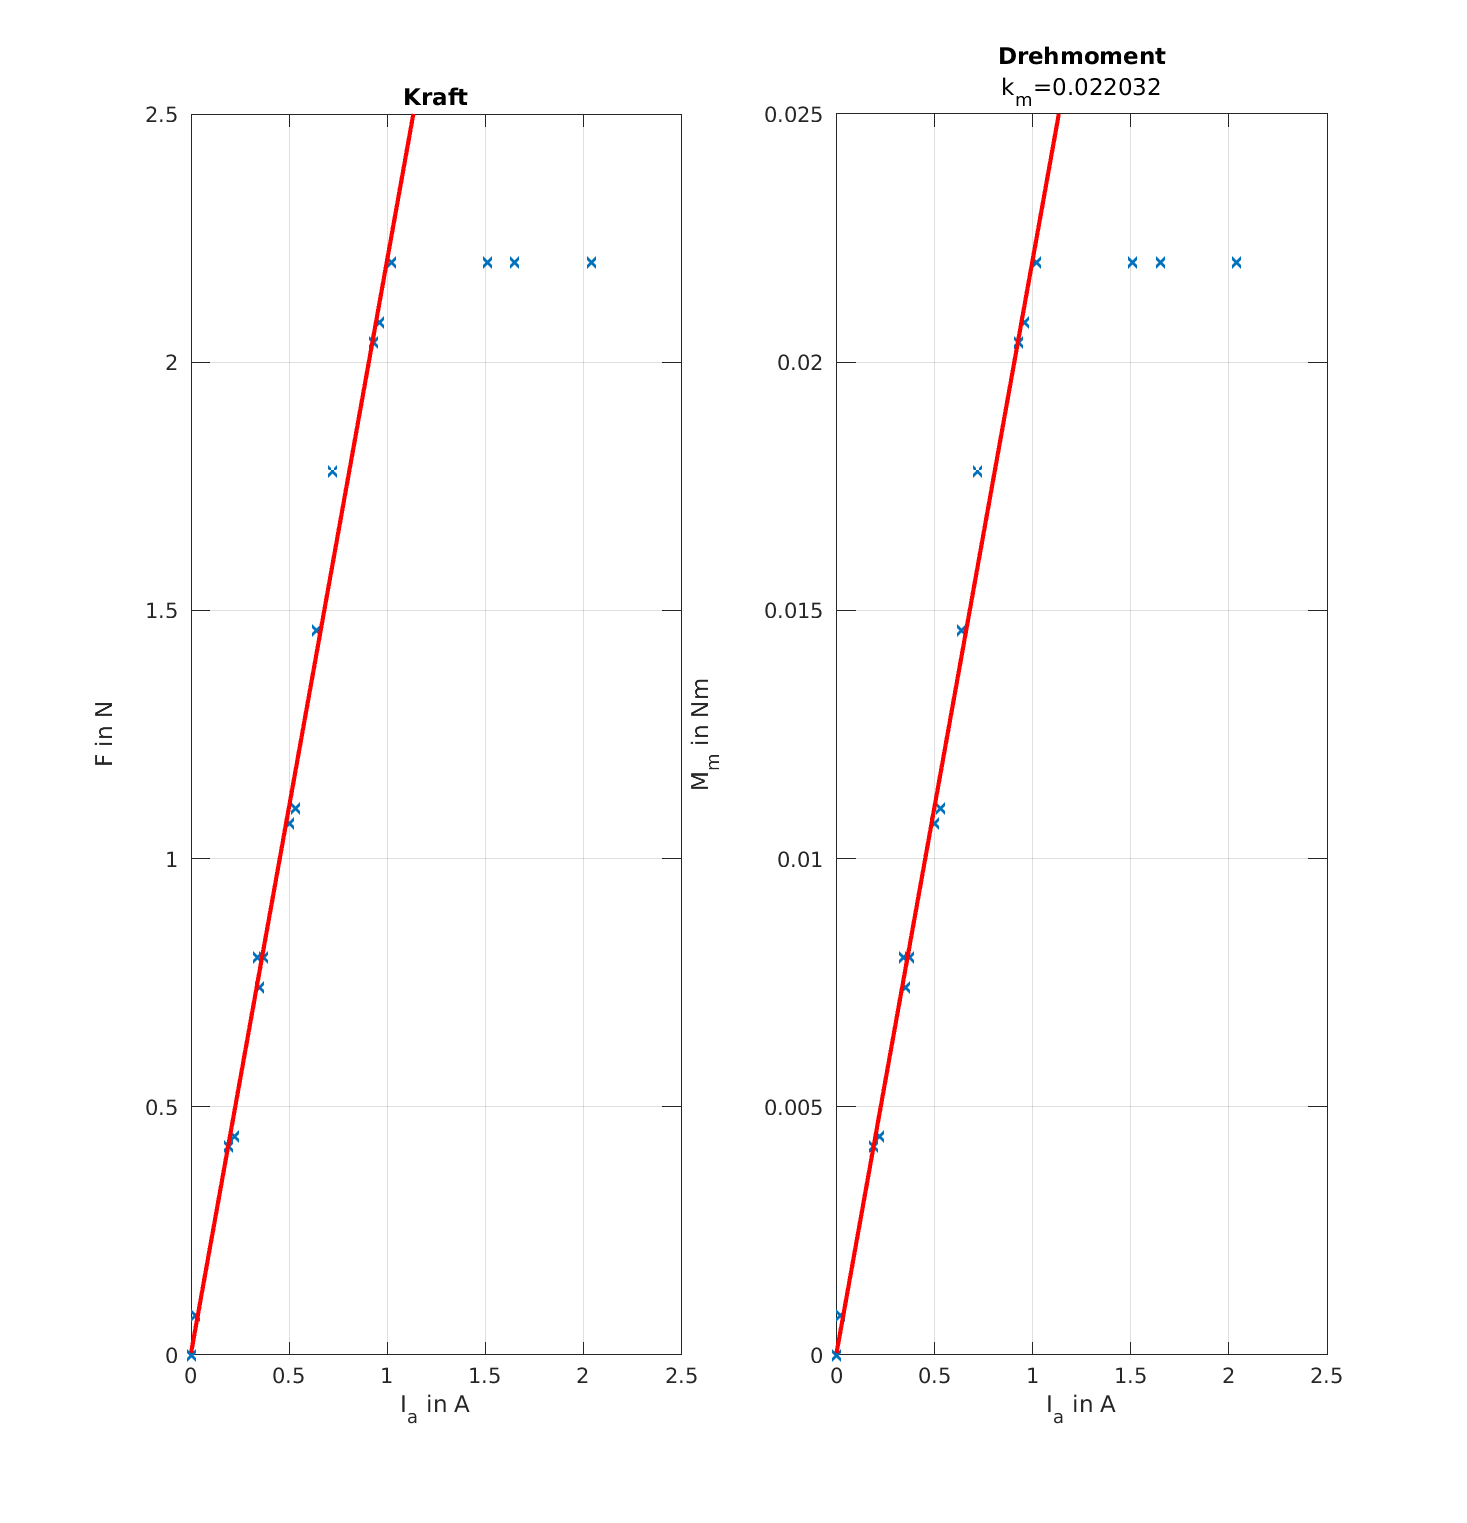
\includegraphics[width=1\textwidth]{as_labor01_1.png}
 \caption{Plot der Aufgabe 1}
 \label{fig:PlotAufgabe1}
\end{figure}

\subsection{Matlab Code}
\lstinputlisting[language=Matlab]{matlab/as_labor01_1.m}

\section{Messung des Ankerwiderstand}

\subsection{Beschreibung}

Im zweiten Versuch soll der Ankerwiderstand $R$ bestimmt werden.
Der Ankerwiderstand kann über das Ohm'sche Gesetz berechnet werden,
dafür ist eine Matrix mit den Messwerten der Spannungen und Ströme gegeben.
Da mit den Messwerten die Ströme über den Spannungen abgebildet werden ist die
Steigung nicht der Widerstand sondern der Leitwert. Deshalb muss zur Ermittlung
des Ankerwiderstand noch das Reziproke des Leitwerts berechnet werden.

\begin{equation} \label{eq121}
    \begin{split}
        R&=\frac{U_a}{I_a} \Leftrightarrow G=\frac{1}{R}=\frac{I_a}{U_a}\\
        R&\simeq 3.26 \mathrm{\Omega}
    \end{split}
\end{equation}

\subsection{Ausgabe der Lösung}
\begin{figure}[H]
 \centering
 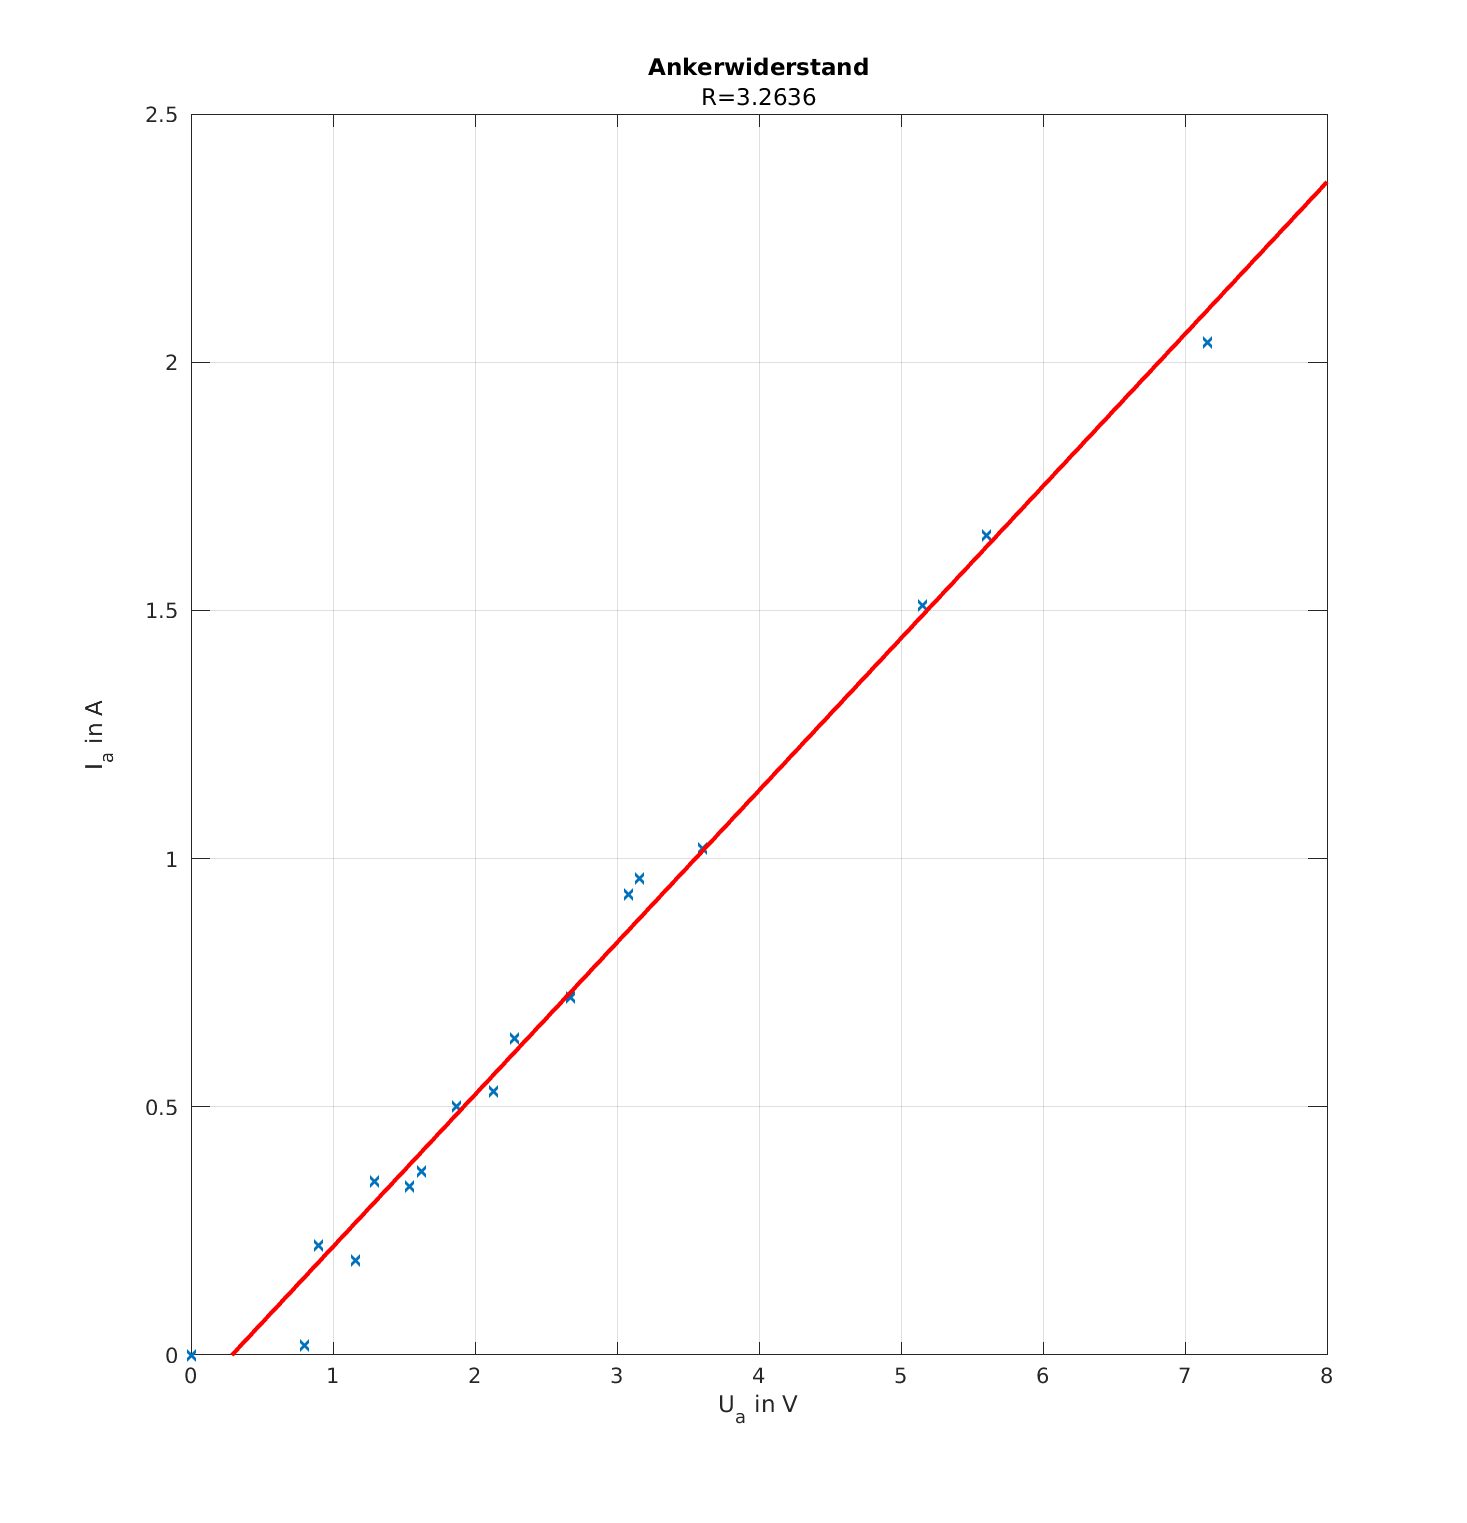
\includegraphics[width=1\textwidth]{as_labor01_2.png}
 \caption{Plot der Aufgabe 2}
 \label{fig:PlotAufgabe2}
\end{figure}

\subsection{Matlab Code}
\lstinputlisting[language=Matlab]{matlab/as_labor01_2.m}

\section{Messung des Stillstandsdrehmomentes}

\subsection{Beschreibung}
\lipsum[1]\\

\subsection{Ausgabe der Lösung}
\begin{figure}[htp]
 \centering
 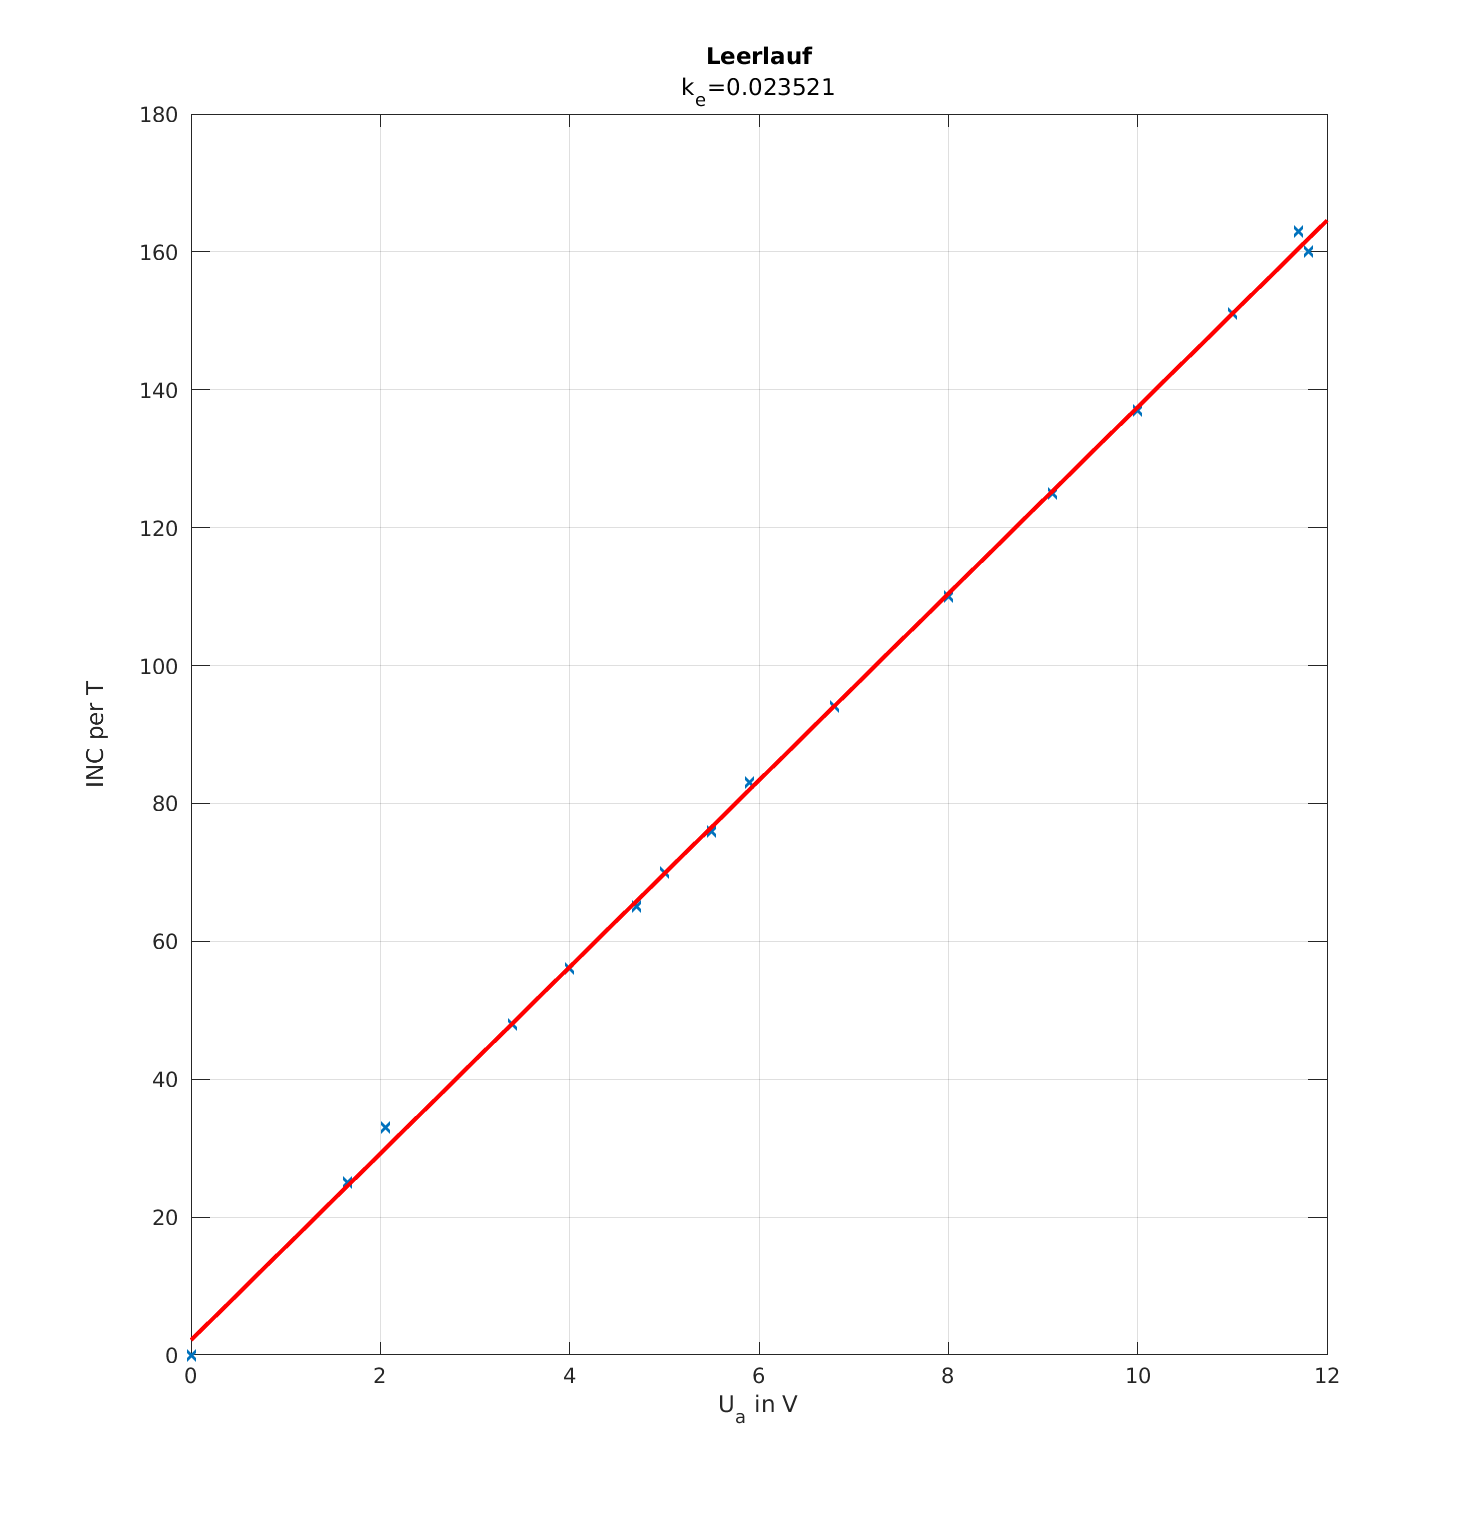
\includegraphics[width=1\textwidth]{as_labor01_3.png}
 \caption{Plot der Aufgabe 3}
 \label{fig:PlotAufgabe3}
\end{figure}

\subsection{Matlab Code}
\lstinputlisting[language=Matlab]{matlab/as_labor01_3.m}

\section{Messung der Kennlinie des Verstärkers}

\subsection{Beschreibung}

In der letzten Messung soll die Kennlinie des Messverstärkers ermittelt
werden und damit der Verstärkungsfaktor $A$ bestimmt werden. Dafür liegt
eine Matrix mit den Eingangsspannungen $U_e$ und den Ausgangspannungen
$U_a$ vor.
Da der Verstärker Ausgangsseitig bei etwa $+13.75\mathrm{V}$ und 
$-13.06\mathrm{V}$ in Sättigung geht, werden die jeweils ersten 2
und die letzten beide Werte nicht betrachtet.

Die Steigung der linearen Funktion ist 

Der Verstärkungsfaktor $A$ ist der Quotient aus Ausgangs- und Eingangsspannung
und somit die Steigung.

\begin{equation} \label{eq141}
    \begin{split}
        A=\frac{U_a}{U_e}\simeq2 \mathrm{V}
    \end{split}
\end{equation}



\subsection{Ausgabe der Lösung}
\begin{figure}[H]
 \centering
 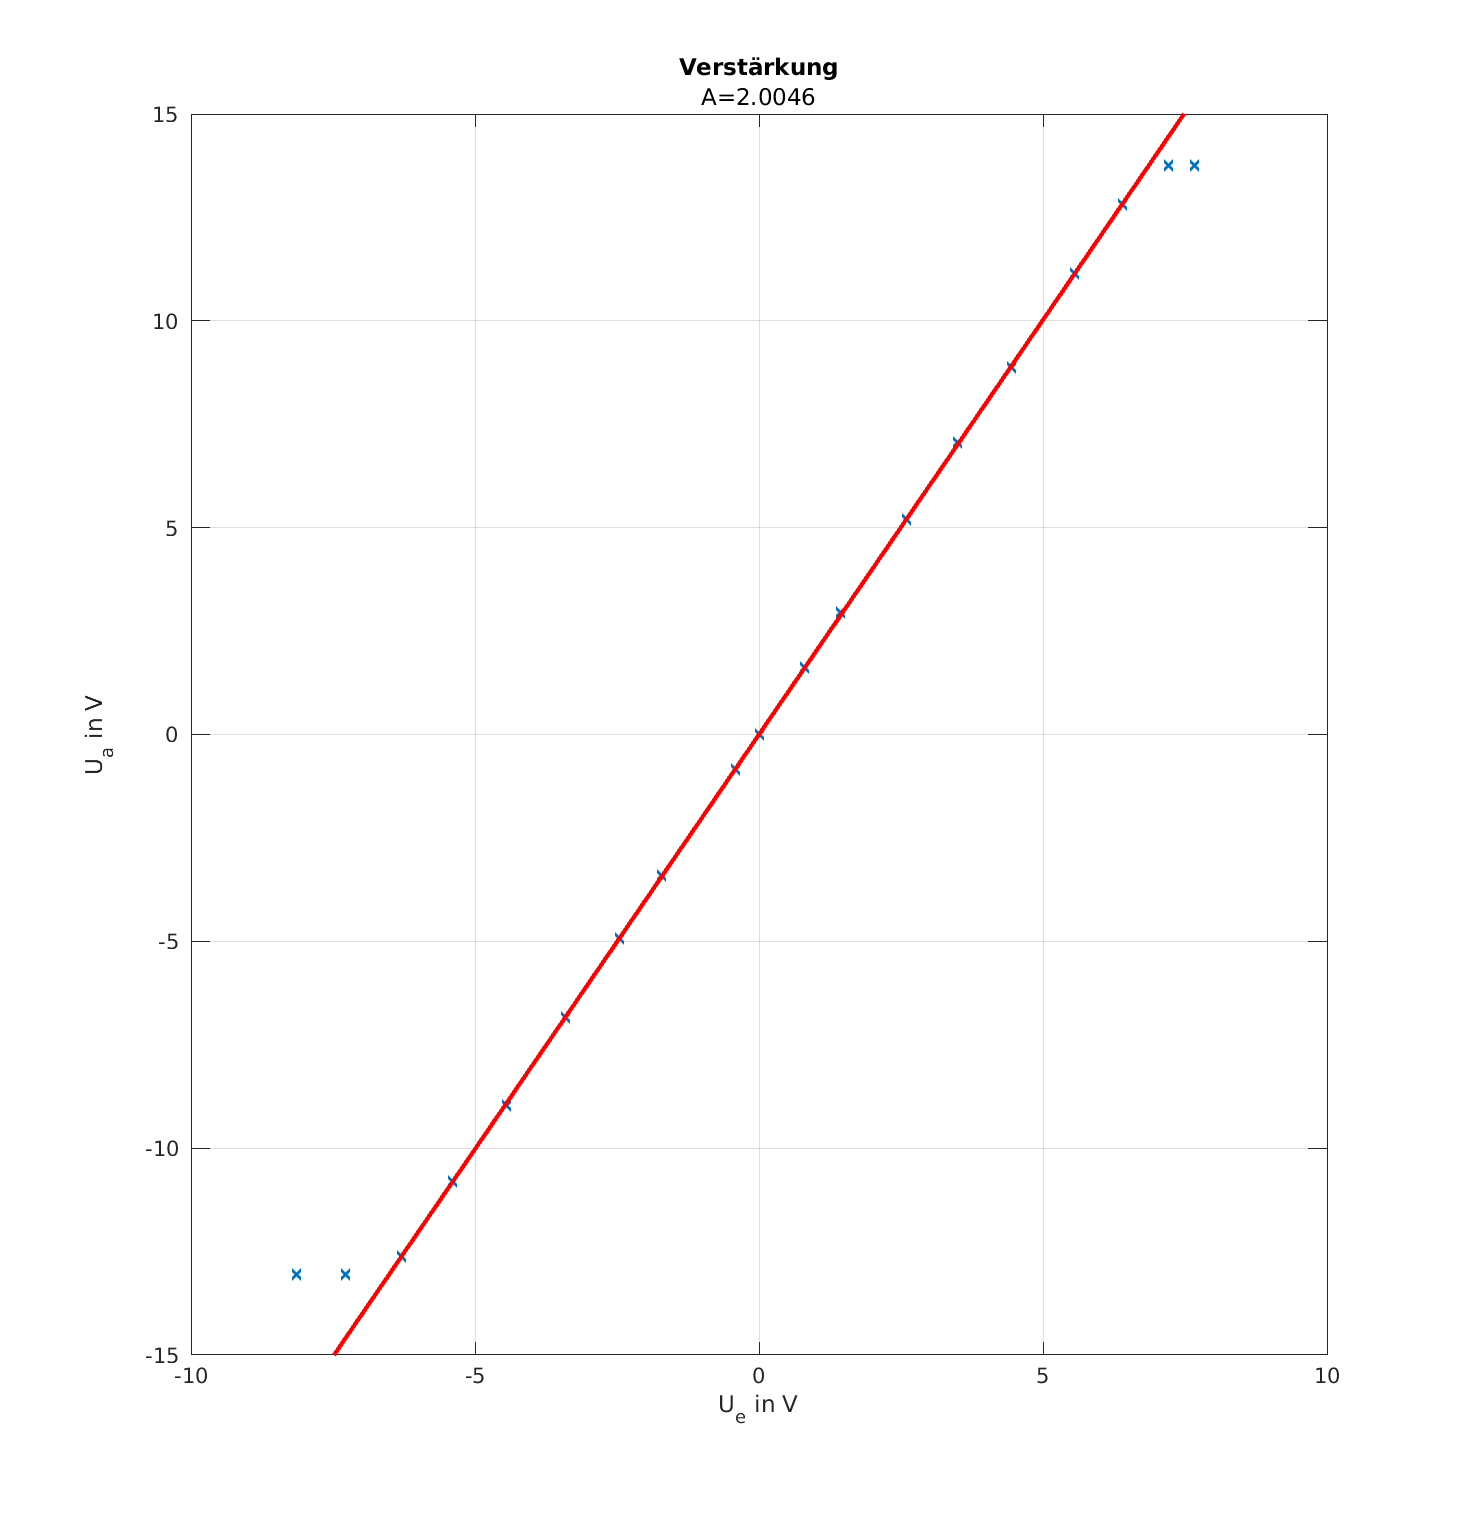
\includegraphics[width=1\textwidth]{as_labor01_4.png}
 \caption{Plot der Aufgabe 4}
 \label{fig:PlotAufgabe4}
\end{figure}

\subsection{Matlab Code}
\lstinputlisting[language=Matlab]{matlab/as_labor01_4.m}


\end{document}

\section{Labor 1}

\subsection{Einleitung und Ziel}

Um später einen permanent erregten Gleichstrommotor zu modellieren, soll
in dieser ersten Laborübung in Aktor und Sensorik die wichtigsten
Kennwerte des Systems bestimmt werden. Dieses sind die Momentenkonstante
$k_M$, der Ankerwiderstand $R$, die Motorkonstante $k_e$ und der
Verstärkungsfaktor $A$ des Messverstärkers. 

Um diese Konstanten zu bestimmen wurden jeweils eine Menge an Messwerten
aufgenommen. Mit diesen wird mittels der Methode der kleinsten Quadrate 
Ausgleichsrechnungen durchgeführt. Dadurch erhalten wir eine lineare
Funktionen aus denen sich die gesuchten Konstanten bestimmen lassen.
\subsection{Grundlagen und Theorie}

\subsubsection{Methode der kleinsten Quadrate}
Die Methode der kleinsten Quadrate ist ein mathematisches Verfahren, bei dem eine lineare Regression
auf der Basis einer Wolke aus Datenpunkten berechnet werden soll. Es soll eine Kurve gefunden werden,
die möglichst nah an den Punkten verläuft. Dazu bestimmt man die Parameter dieser Kurve numerisch, indem die Summe 
der quadratischen Abweichungen der Kurve von den beobachteten Punkten minimiert wird.

Zur Umsetzung der Methode der kleinsten Quadrate in Matlab werden die Funktionen polyfit() und polyval() verwendet. 
polyfit() erhält beim Aufruf die Werte der Punktwolke sowie den Grad des Polynoms und gibt die entsprechenden Koeffizienten
zurück. polyval() ermittelt aus den Koeffizienten und den x-Werten die tatsächlichen Werte, mit welchen die Kurve geplottet 
werden kann. 

\subsubsection{Inkrementalgeber}
Ein Inkrementalgeber ist ein Messinstrument zur Ermittlung von Lage- oder Winkeländerung (bei rotierenden Objekten). 
Als verschiedene Arten wird zwischen der photoelektrischen Abtastung (entweder als abbildendes oder interferentielles
Messprinzip), der magnetischen Abtastung und per Schleifkontakt unterschieden. Dabei werden zwei um 90 Grad verschobene
Signale erzeugt, über die sich Drehgeschwindigkeit, -richtung und -winkel bestimmen lassen.
Im Beispielt der photoelektrischen Abtastung wird eine Drehscheibe verwendet, die mit mehreren Schlitzen unterteilt ist und 
zwischen einer Leuchtdiode und zwei leicht versetzten Photodetektoren angebracht ist. Wenn sich die Scheibe dreht, zählen
die Photodetektoren die Impulse, welche von Leuchtdiode und Lichtgitter der Drehscheibe entstehen.  
\subsection{Aufgabenstellung und Versuch}

\subsubsection{Messung des Stillstandsdrehmomentes}

Im ersten Versuch soll die Momentenkonstante $k_m$ bestimmt werden.
Sie hängt folgendermaßen mit dem Drehmoment $M_M$ und dem Motorstrom $i_a(t)$
zusammen. 

\begin{equation} \label{eq111}
    \begin{split}
        M_M(t)&=k_m \cdot i_a(t)\\
        k_m&=\frac{M_M(t)}{i_a(t)}
    \end{split}
\end{equation}

Als Messwerte ist eine Matrix mit den Motorströmen $I_a$ und der Auslenkungskraft $F$
gegeben. Um daraus das Drehmoment $M_M$ zu bestimmen wird der Radius $r$ benötigt,
welcher mit $1 \mathrm{cm}$ gegeben ist.

\begin{equation} \label{eq112}
    \begin{split}
        M_M&=r \cdot F \\
        k_m&=\frac{r\cdot F(t)}{i_a(t)}
    \end{split}
\end{equation}

Anschließend kann die Momentenkonstante $k_m$ über die Steigung der geplotteten
Gerade bestimmt werden. Hierfür muss gewährleistet werden, dass der Arbeistpunkt
linear ist. Deshalb dürfen die letzten drei Messwerte in der linearen Regression
nicht betrachtet werden.

\begin{equation} \label{eq113}
    \begin{split}
        k_m\simeq 0.022 \mathrm{\frac{Nm}{A}}
    \end{split}
\end{equation}

\begin{figure}[H]
 \centering
 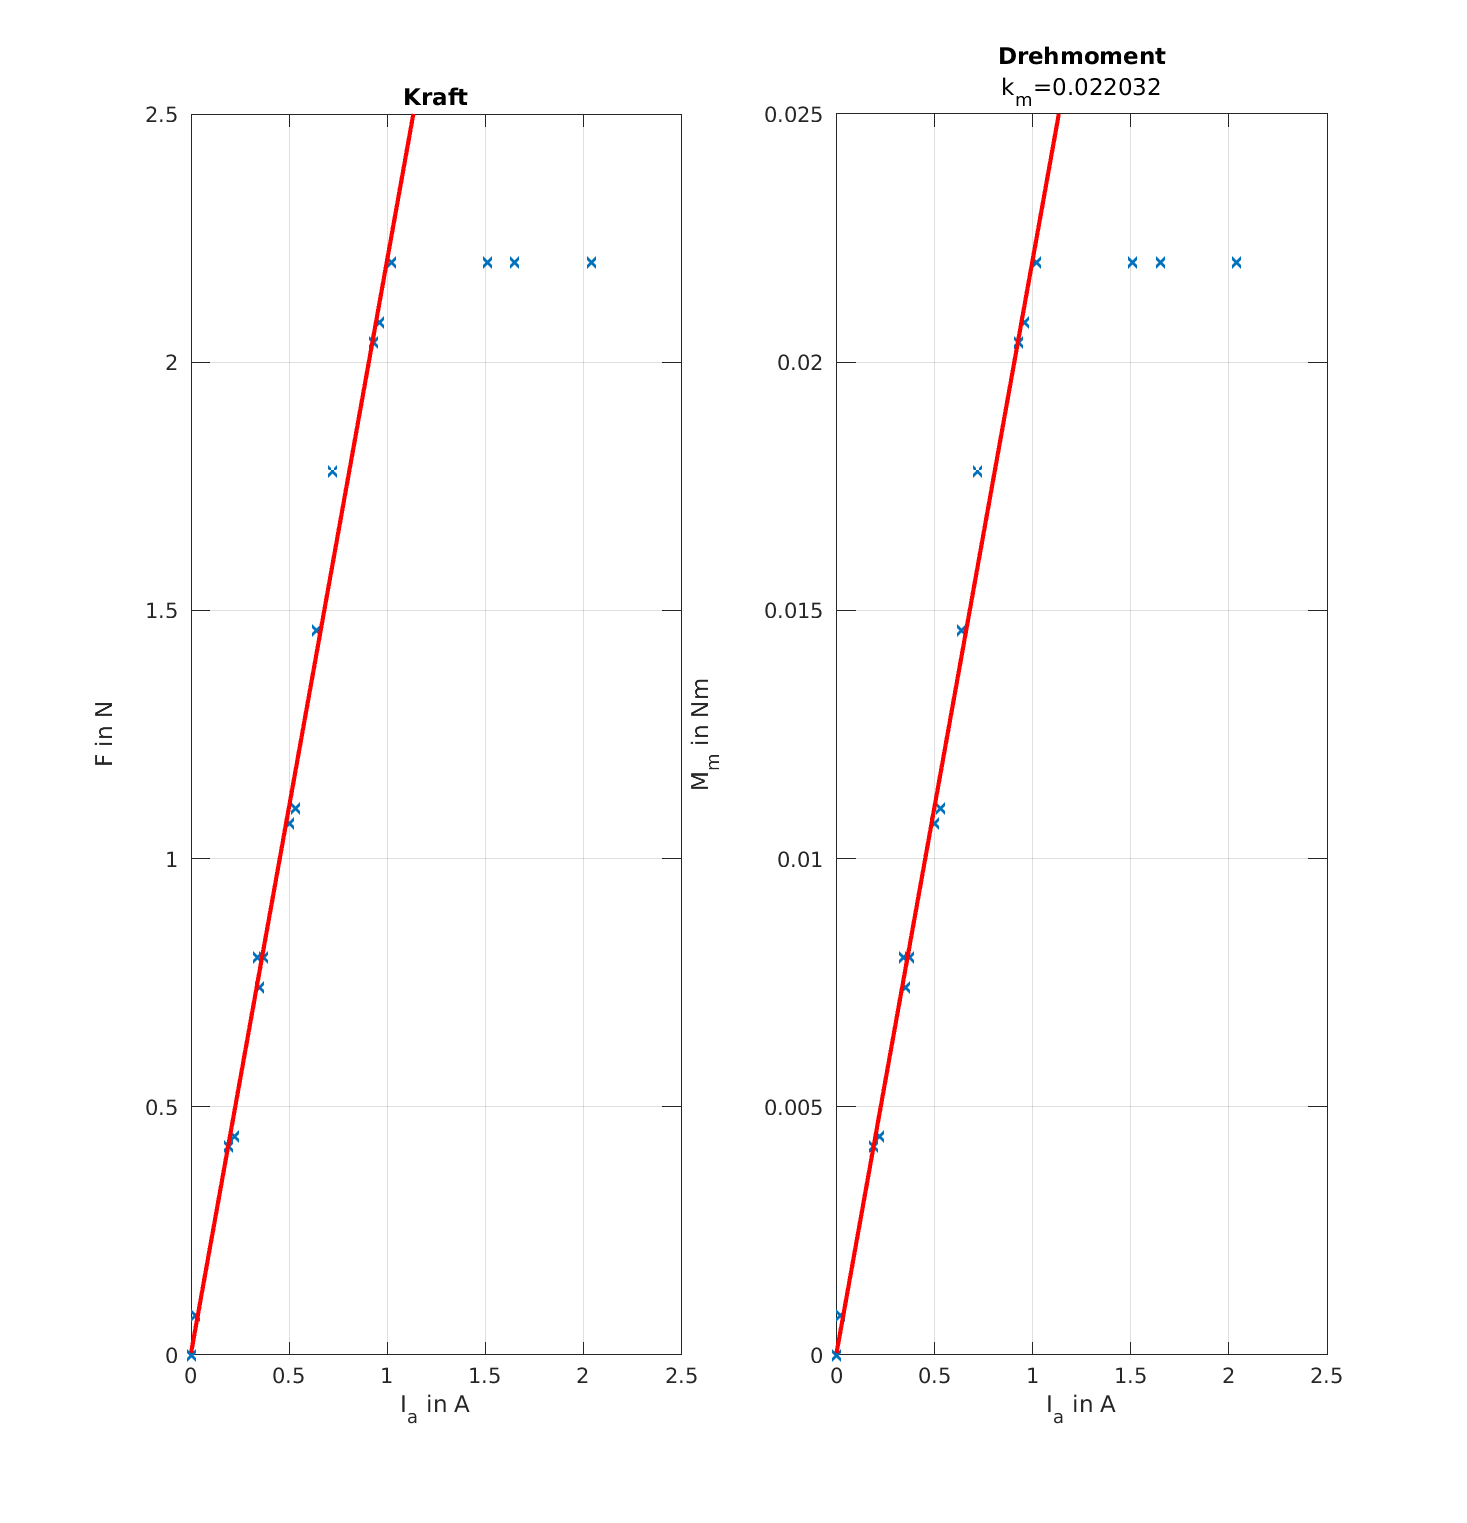
\includegraphics[width=1\textwidth]{as_labor01_1.png}
 \caption{Plot der Aufgabe 1}
 \label{fig:PlotAufgabe1}
\end{figure}
\subsubsection{Messung des Ankerwiderstand}

Im zweiten Versuch soll der Ankerwiderstand $R$ bestimmt werden.
Der Ankerwiderstand kann über das Ohm'sche Gesetz berechnet werden,
dafür ist eine Matrix mit den gemessenen Messwerten der Spannungen
und Ströme gegeben.

Da mit den Messwerten die Ströme über den Spannungen abgebildet werden ist die
Steigung nicht der Widerstand sondern der Leitwert. Deshalb muss zur Ermittlung
des Ankerwiderstand noch das Reziproke des Leitwerts berechnet werden.

\begin{equation} \label{eq121}
    \begin{split}
        R&=\frac{U_a}{I_a} \Leftrightarrow G=\frac{1}{R}=\frac{I_a}{U_a}\\
        R&\simeq 3.26 \mathrm{\Omega}
    \end{split}
\end{equation}

\begin{figure}[H]
 \centering
 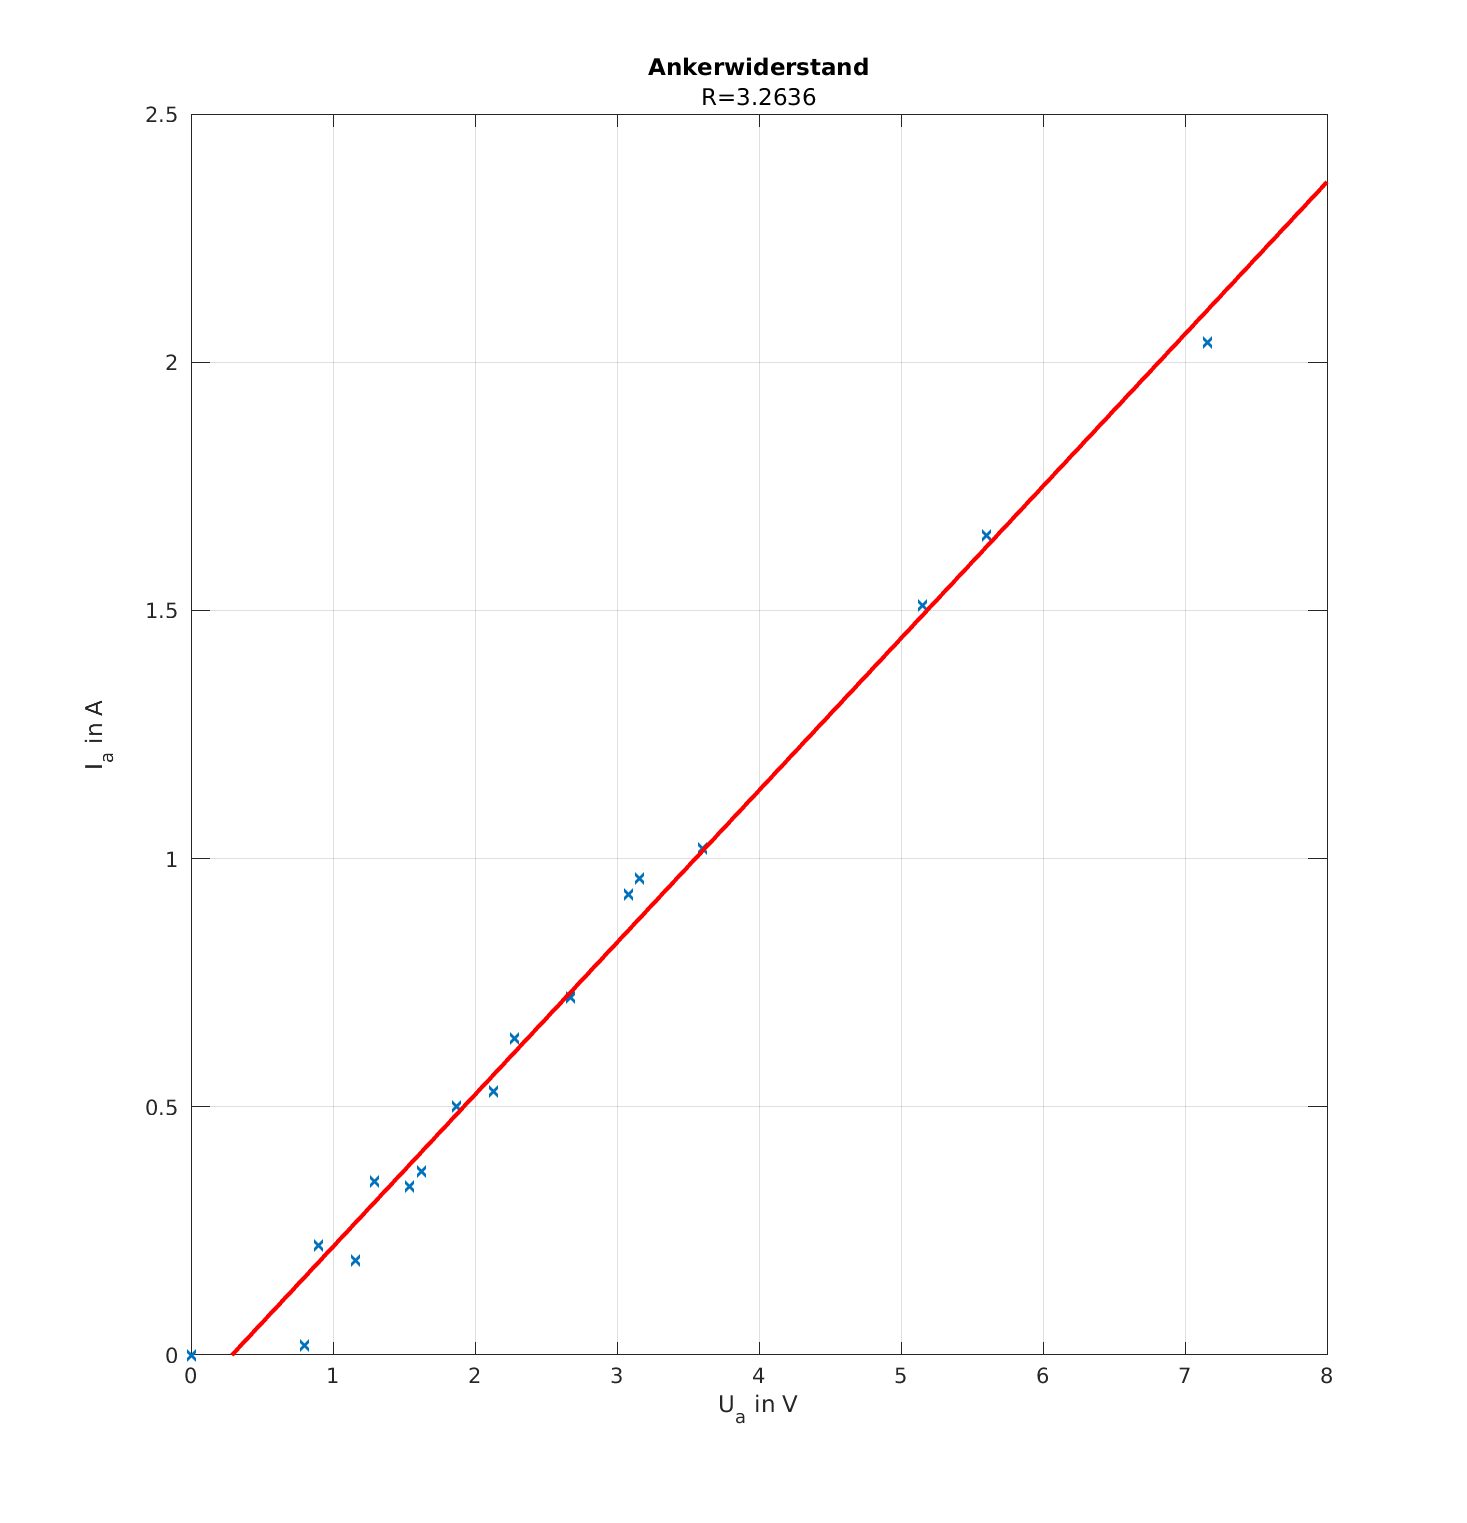
\includegraphics[width=1\textwidth]{as_labor01_2.png}
 \caption{Plot der Aufgabe 2}
 \label{fig:PlotAufgabe2}
\end{figure}
\subsubsection{Messung des Stillstandsdrehmomentes}

Im dritten Versuch soll die Konstante $k_e$ bestimmt werden. Diese
beschreibt als Proportionalfaktor den Zusammengang zwischen der
induzierten Spannung $U_i$ und der Winkelgeschwindigkeit $\omega$.

\begin{equation} \label{eq131}
    \begin{split}
        u_i(t)=k_e \cdot \omega (t)
    \end{split}
\end{equation}

Gegeben sind in dieser Aufgabe sind die Messwerte in einer Matrix. Diese
enthält die Spannungswerten von $U_a=U_i$, welche mit einem Multimeter
gemessen worden sind und den Inkrementen pro $\mathrm{ms}$ $Y$, ermittelt
durch einen Inkrementalgeber und einen Mikrocontroller.

Um $k_e$ zu bestimmen wird neben der direkt gegebenen Spannung $U_a$ auch
die Winkelgeschwindigkeit $\omega$ benötigt. Diese ist das Produkt aus
$2\pi$ und der Drehzahl $n$. Während die Winkelgeschwindigkeit angibt wie
schnell sich ein Winkel mit der Zeit um eine Achse ändert, gibt die Drehzahl
die Anzahl der Umdrehungen in einer Zeitspanne an.

\begin{equation} \label{eq132}
    \begin{split}
        k_e = \frac{U_a}{\omega}= \frac{U_a}{2 \pi n}
    \end{split}
\end{equation}

Die gemessen Inkremente pro Zeit müssen daher umgerechnet werden. Diese
wurden mit dem C167 Mikrocontroller mit einer Abtastzeit $T=1\mathrm{ms}$
aufgenommen. Der Inkrementalgeber besitzt 500 Inkremente pro Umdrehung.
Durch eine Vierfachauswertung ergeben sich $P_z=\frac{2000}{2\pi} \mathrm{\frac{INK}{rad}}$.
Dadurch ergibt sich folgender Umrechnungsfaktor $\lambda$.

\begin{equation} \label{eq133}
    \begin{split}
        \lambda = \frac{1000}{P_z} \mathrm{\frac{ms}{s} \frac{rad}{INK}}
    \end{split}
\end{equation}

Über diesen Faktor lässt sich die Drehzahl bestimmen, damit die
Winkelgeschwindigkeit und abschließend auch $k_e$.

\begin{equation} \label{eq133}
    \begin{split}
        n &= \lambda \cdot Y \qquad \text{in} \mathrm{\frac{rad}{s}}\\
        \omega &= 2 \pi \lambda \cdot Y \qquad \text{in} \mathrm{\frac{rad}{s}}\\
        k_e &= \frac{U_a}{2 \pi \lambda \cdot Y}  \qquad \text{in} \mathrm{\frac{Vs}{rad}}
    \end{split}
\end{equation}

Dadurch berechnet sich $ke$ nach über das Reziproke der Steigung der Funktion
multipliziert mit dem Faktor $\lambda$.

\begin{equation} \label{eq134}
    \begin{split}
    k_e = \frac{1}{m \cdot \lambda} \simeq 0.0235 \mathrm{\frac{Vs}{rad}}
    \end{split}
\end{equation}

\begin{figure}[H]
 \centering
 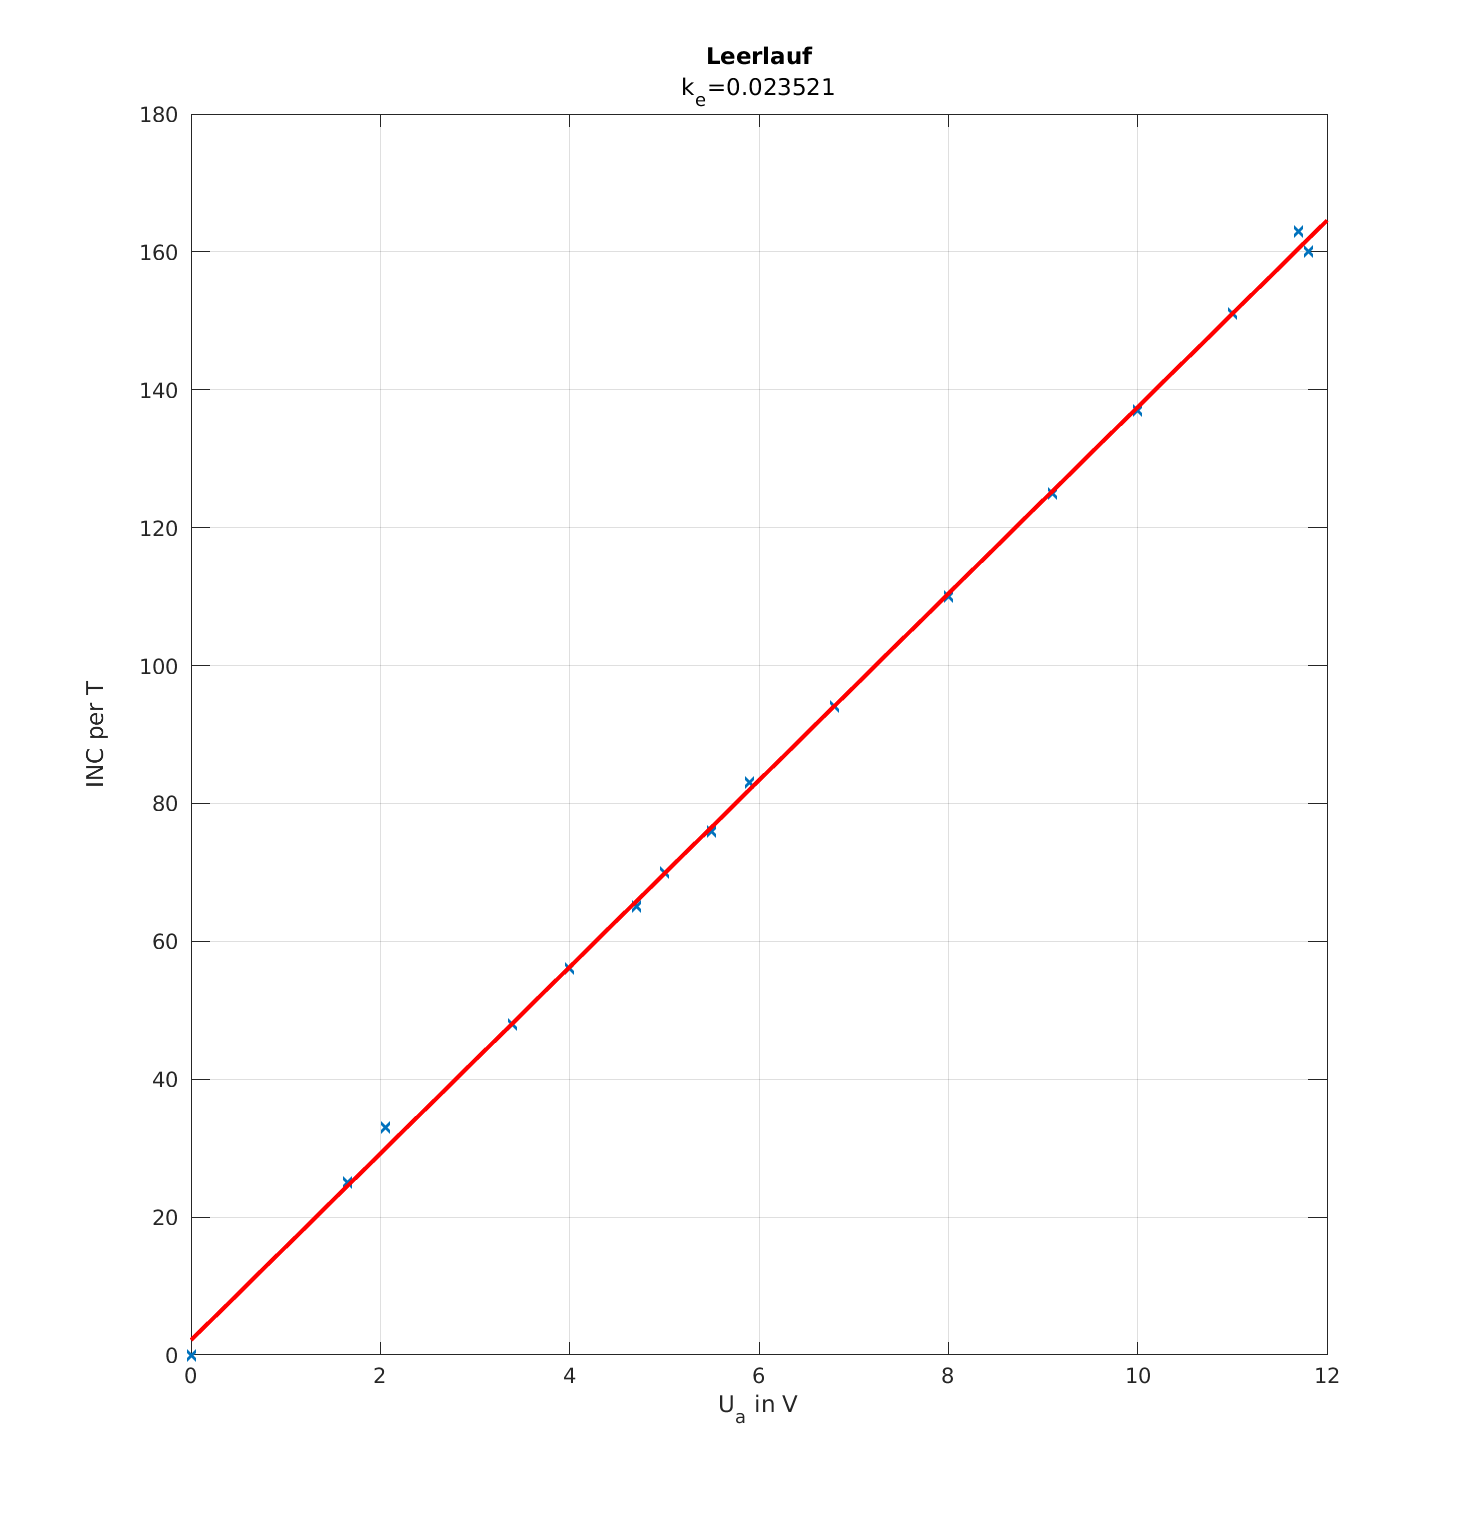
\includegraphics[width=1\textwidth]{as_labor01_3.png}
 \caption{Plot der Aufgabe 3}
 \label{fig:PlotAufgabe3}
\end{figure}
\subsubsection{Messung der Kennlinie des Verstärkers}

In der letzten Messung soll die Kennlinie des Messverstärkers ermittelt
werden und damit der Verstärkungsfaktor $A$ bestimmt werden. Dafür liegt
eine Matrix mit den Eingangsspannungen $U_e$ und den Ausgangspannungen
$U_a$ vor. Da der Verstärker ausgangsseitig bei etwa $+13.75\mathrm{V}$
und $-13.06\mathrm{V}$ in Sättigung geht, werden die jeweils ersten beiden
und die letzten beiden Messwerte für die Berechnung der Funktion nicht
betrachtet.

Der Verstärkungsfaktor $A$ ist der Quotient aus Ausgangs- und Eingangsspannung
und somit die Steigung der ermittelten Funktion.

\begin{equation} \label{eq141}
    \begin{split}
        A=\frac{U_a}{U_e}\simeq2 \mathrm{V}
    \end{split}
\end{equation}

\begin{figure}[H]
 \centering
 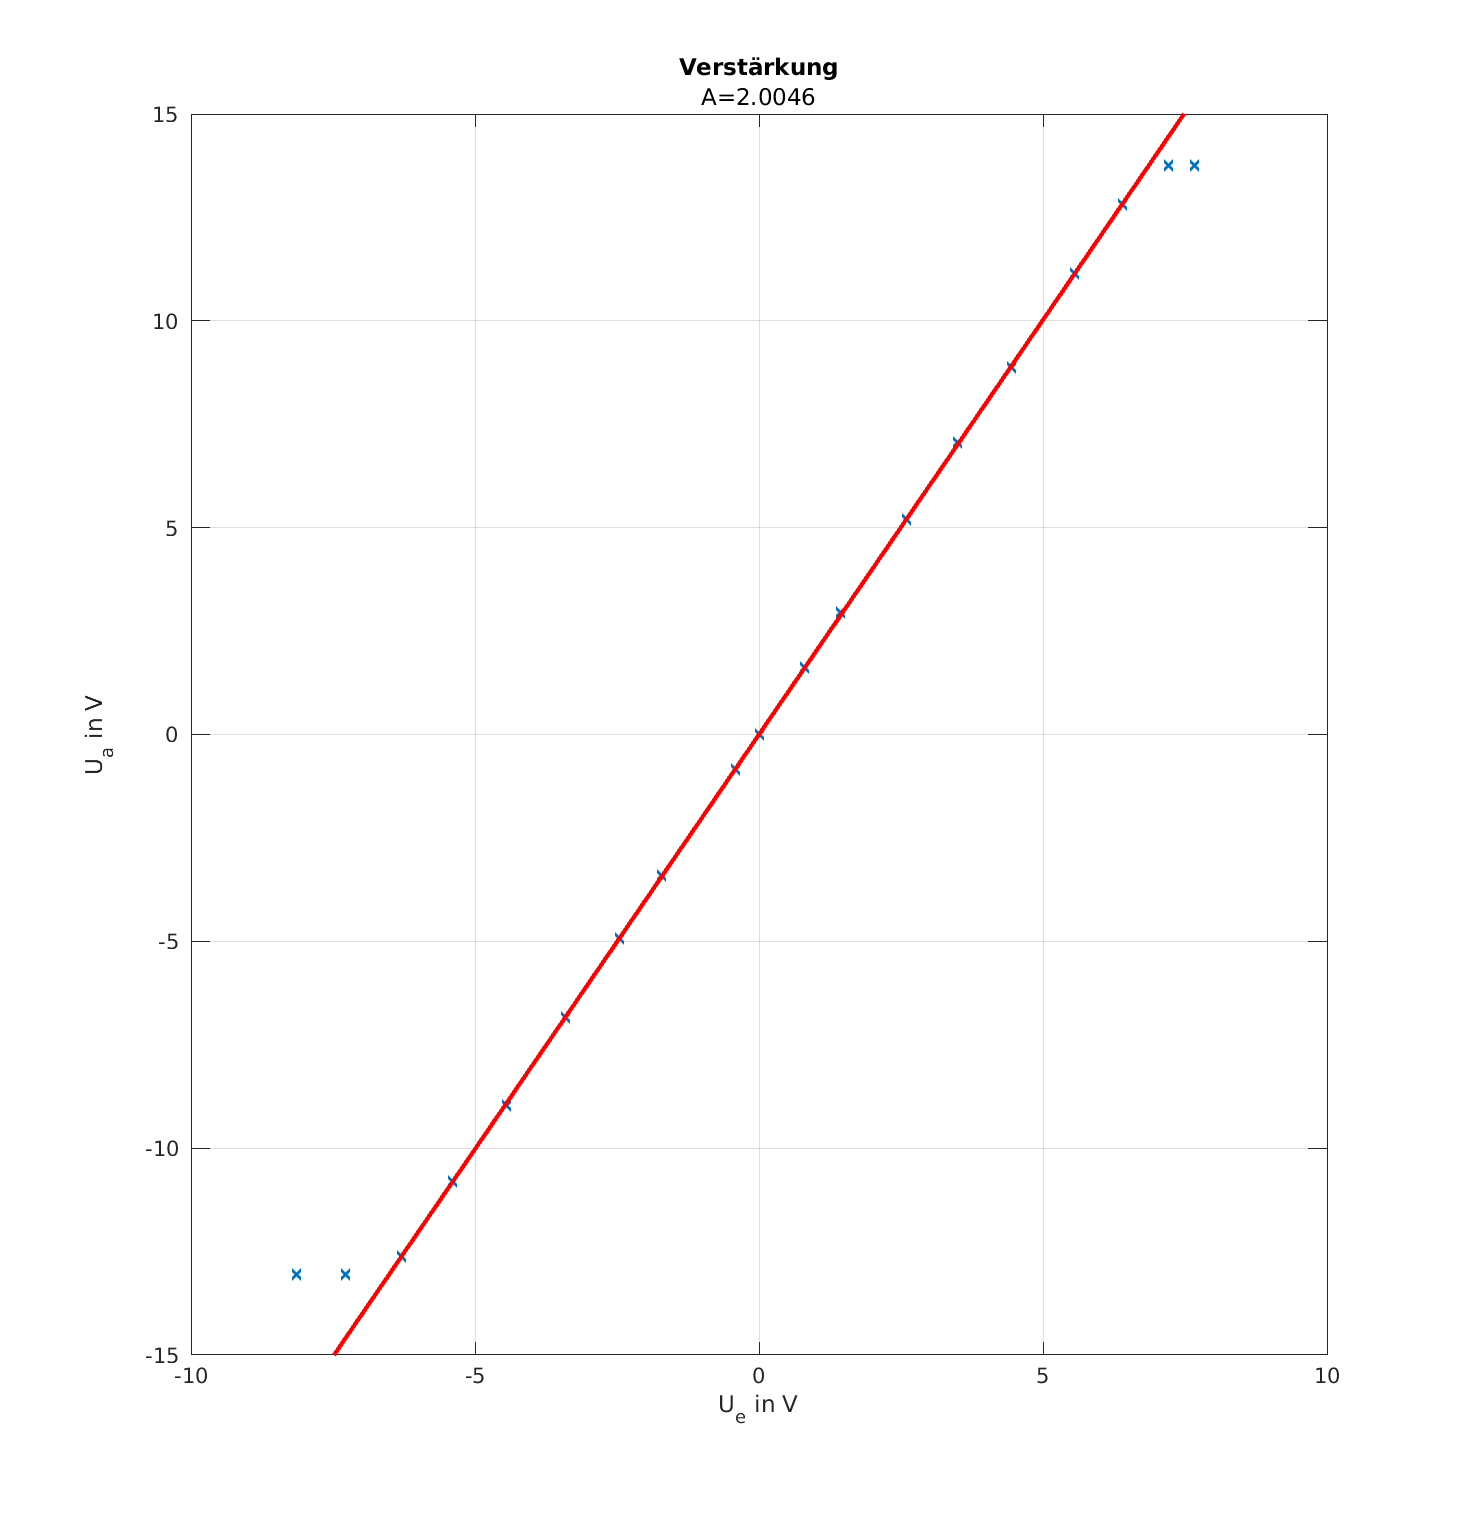
\includegraphics[width=1\textwidth]{as_labor01_4.png}
 \caption{Plot der Aufgabe 4}
 \label{fig:PlotAufgabe4}
\end{figure}
%\subsection{Zusammenfassung}
\subsection{Anhang}

\subsubsection{Aufgabenbeschreibung}
\begin{figure}[H]
    \centering
    \includegraphics[page=3, width=0.8\textwidth]{../Aufgabenstellung.pdf}
    %\caption{Aufbau der CBM-Toolchain}
    \label{fig:Aufgabenstellung A1}
\end{figure}

\begin{figure}[H]
    \centering
    \includegraphics[page=4, width=0.8\textwidth]{../Aufgabenstellung.pdf}
    %\caption{Aufbau der CBM-Toolchain}
    \label{fig:Aufgabenstellung A1}
\end{figure}

\subsubsection{Matlab Code}
\lstinputlisting[language=Matlab]{matlab/as_labor01_1.m}
\lstinputlisting[language=Matlab]{matlab/as_labor01_2.m}
\lstinputlisting[language=Matlab]{matlab/as_labor01_3.m}
\lstinputlisting[language=Matlab]{matlab/as_labor01_4.m}

%\subsubsection{Messwerte}



% % !TEX root = ./main.tex

\documentclass{article}
\usepackage[utf8]{inputenc}
\usepackage[ngerman]{babel}
\usepackage{pdfpages}
\usepackage{graphicx}
\usepackage{amsmath}
\graphicspath{ {./img/} }

\usepackage{lipsum}
\usepackage{float}
\usepackage{listings}

\usepackage{xcolor}

\definecolor{codegreen}{rgb}{0,0.6,0}
\definecolor{codegray}{rgb}{0.5,0.5,0.5}
\definecolor{codepurple}{rgb}{0.58,0,0.82}
\definecolor{backcolour}{rgb}{0.95,0.95,0.92}

\lstdefinestyle{mystyle}{
    backgroundcolor=\color{backcolour},   
    commentstyle=\color{codegreen},
    keywordstyle=\color{magenta},
    numberstyle=\tiny\color{codegray},
    stringstyle=\color{codepurple},
    basicstyle=\ttfamily\footnotesize,
    breakatwhitespace=false,         
    breaklines=true,                 
    captionpos=b,                    
    keepspaces=true,                 
    numbers=left,                    
    numbersep=5pt,                  
    showspaces=false,                
    showstringspaces=false,
    showtabs=false,                  
    tabsize=2
}

\lstset{style=mystyle}
\lstset{literate=%
{Ö}{{\"O}}1
{Ä}{{\"A}}1
{Ü}{{\"U}}1
{ß}{{\ss}}2
{ü}{{\"u}}1
{ä}{{\"a}}1
{ö}{{\"o}}1
}

\newcommand{\nr}{1}


\title{Aktorik Sensorik \\ Labor 1}
\author{Anton Kress (S872899), Jan Abel (S876662)}
\date{October 2020}

\begin{document}

\maketitle

\newpage
\tableofcontents 
\section{Labor 1}

\subsection{Einleitung und Ziel}

Um später einen permanent erregten Gleichstrommotor zu modellieren, soll
in dieser ersten Laborübung in Aktor und Sensorik die wichtigsten
Kennwerte des Systems bestimmt werden. Dieses sind die Momentenkonstante
$k_M$, der Ankerwiderstand $R$, die Motorkonstante $k_e$ und der
Verstärkungsfaktor $A$ des Messverstärkers. 

Um diese Konstanten zu bestimmen wurden jeweils eine Menge an Messwerten
aufgenommen. Mit diesen wird mittels der Methode der kleinsten Quadrate 
Ausgleichsrechnungen durchgeführt. Dadurch erhalten wir eine lineare
Funktionen aus denen sich die gesuchten Konstanten bestimmen lassen.
\subsection{Grundlagen und Theorie}

\subsubsection{Methode der kleinsten Quadrate}
Die Methode der kleinsten Quadrate ist ein mathematisches Verfahren, bei dem eine lineare Regression
auf der Basis einer Wolke aus Datenpunkten berechnet werden soll. Es soll eine Kurve gefunden werden,
die möglichst nah an den Punkten verläuft. Dazu bestimmt man die Parameter dieser Kurve numerisch, indem die Summe 
der quadratischen Abweichungen der Kurve von den beobachteten Punkten minimiert wird.

Zur Umsetzung der Methode der kleinsten Quadrate in Matlab werden die Funktionen polyfit() und polyval() verwendet. 
polyfit() erhält beim Aufruf die Werte der Punktwolke sowie den Grad des Polynoms und gibt die entsprechenden Koeffizienten
zurück. polyval() ermittelt aus den Koeffizienten und den x-Werten die tatsächlichen Werte, mit welchen die Kurve geplottet 
werden kann. 

\subsubsection{Inkrementalgeber}
Ein Inkrementalgeber ist ein Messinstrument zur Ermittlung von Lage- oder Winkeländerung (bei rotierenden Objekten). 
Als verschiedene Arten wird zwischen der photoelektrischen Abtastung (entweder als abbildendes oder interferentielles
Messprinzip), der magnetischen Abtastung und per Schleifkontakt unterschieden. Dabei werden zwei um 90 Grad verschobene
Signale erzeugt, über die sich Drehgeschwindigkeit, -richtung und -winkel bestimmen lassen.
Im Beispielt der photoelektrischen Abtastung wird eine Drehscheibe verwendet, die mit mehreren Schlitzen unterteilt ist und 
zwischen einer Leuchtdiode und zwei leicht versetzten Photodetektoren angebracht ist. Wenn sich die Scheibe dreht, zählen
die Photodetektoren die Impulse, welche von Leuchtdiode und Lichtgitter der Drehscheibe entstehen.  
\subsection{Aufgabenstellung und Versuch}

\subsubsection{Messung des Stillstandsdrehmomentes}

Im ersten Versuch soll die Momentenkonstante $k_m$ bestimmt werden.
Sie hängt folgendermaßen mit dem Drehmoment $M_M$ und dem Motorstrom $i_a(t)$
zusammen. 

\begin{equation} \label{eq111}
    \begin{split}
        M_M(t)&=k_m \cdot i_a(t)\\
        k_m&=\frac{M_M(t)}{i_a(t)}
    \end{split}
\end{equation}

Als Messwerte ist eine Matrix mit den Motorströmen $I_a$ und der Auslenkungskraft $F$
gegeben. Um daraus das Drehmoment $M_M$ zu bestimmen wird der Radius $r$ benötigt,
welcher mit $1 \mathrm{cm}$ gegeben ist.

\begin{equation} \label{eq112}
    \begin{split}
        M_M&=r \cdot F \\
        k_m&=\frac{r\cdot F(t)}{i_a(t)}
    \end{split}
\end{equation}

Anschließend kann die Momentenkonstante $k_m$ über die Steigung der geplotteten
Gerade bestimmt werden. Hierfür muss gewährleistet werden, dass der Arbeistpunkt
linear ist. Deshalb dürfen die letzten drei Messwerte in der linearen Regression
nicht betrachtet werden.

\begin{equation} \label{eq113}
    \begin{split}
        k_m\simeq 0.022 \mathrm{\frac{Nm}{A}}
    \end{split}
\end{equation}

\begin{figure}[H]
 \centering
 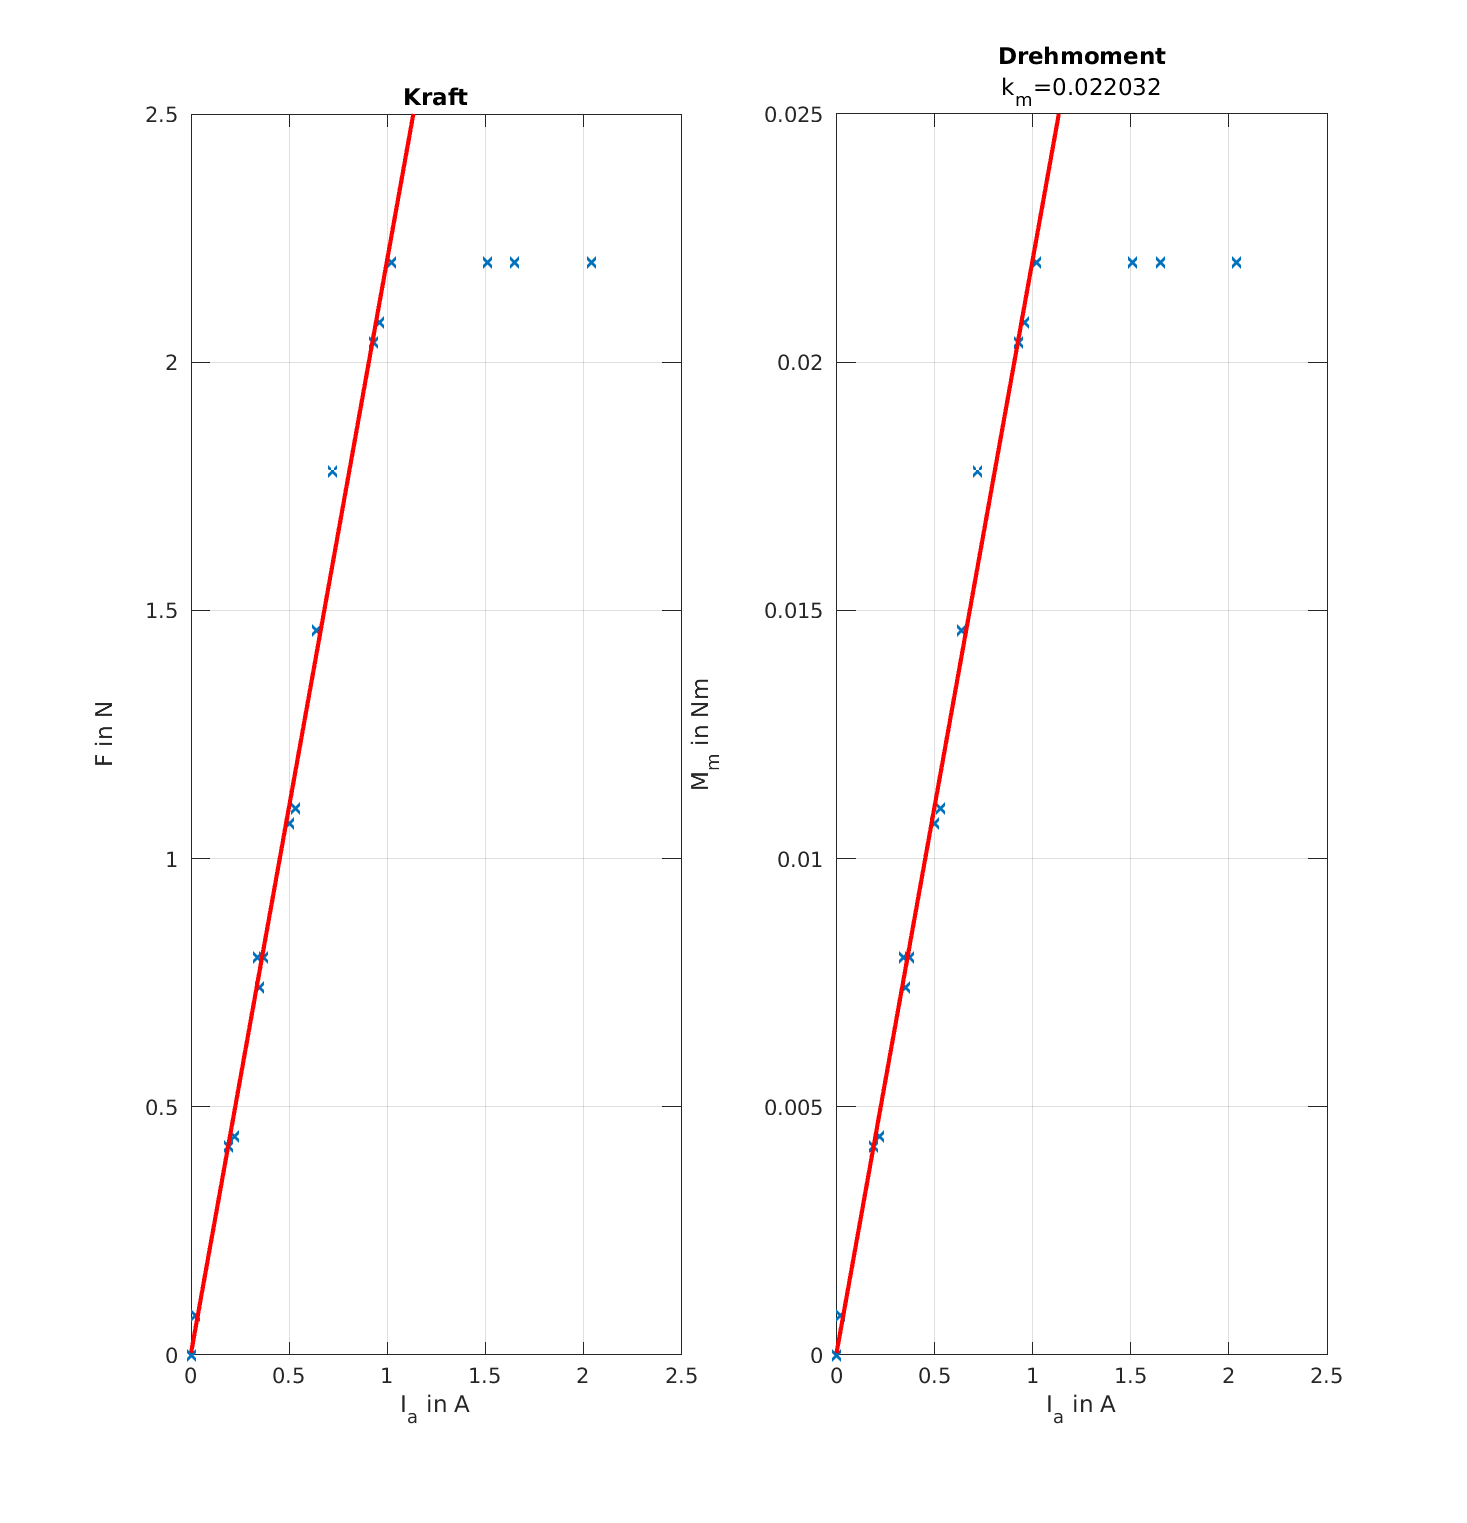
\includegraphics[width=1\textwidth]{as_labor01_1.png}
 \caption{Plot der Aufgabe 1}
 \label{fig:PlotAufgabe1}
\end{figure}
\subsubsection{Messung des Ankerwiderstand}

Im zweiten Versuch soll der Ankerwiderstand $R$ bestimmt werden.
Der Ankerwiderstand kann über das Ohm'sche Gesetz berechnet werden,
dafür ist eine Matrix mit den gemessenen Messwerten der Spannungen
und Ströme gegeben.

Da mit den Messwerten die Ströme über den Spannungen abgebildet werden ist die
Steigung nicht der Widerstand sondern der Leitwert. Deshalb muss zur Ermittlung
des Ankerwiderstand noch das Reziproke des Leitwerts berechnet werden.

\begin{equation} \label{eq121}
    \begin{split}
        R&=\frac{U_a}{I_a} \Leftrightarrow G=\frac{1}{R}=\frac{I_a}{U_a}\\
        R&\simeq 3.26 \mathrm{\Omega}
    \end{split}
\end{equation}

\begin{figure}[H]
 \centering
 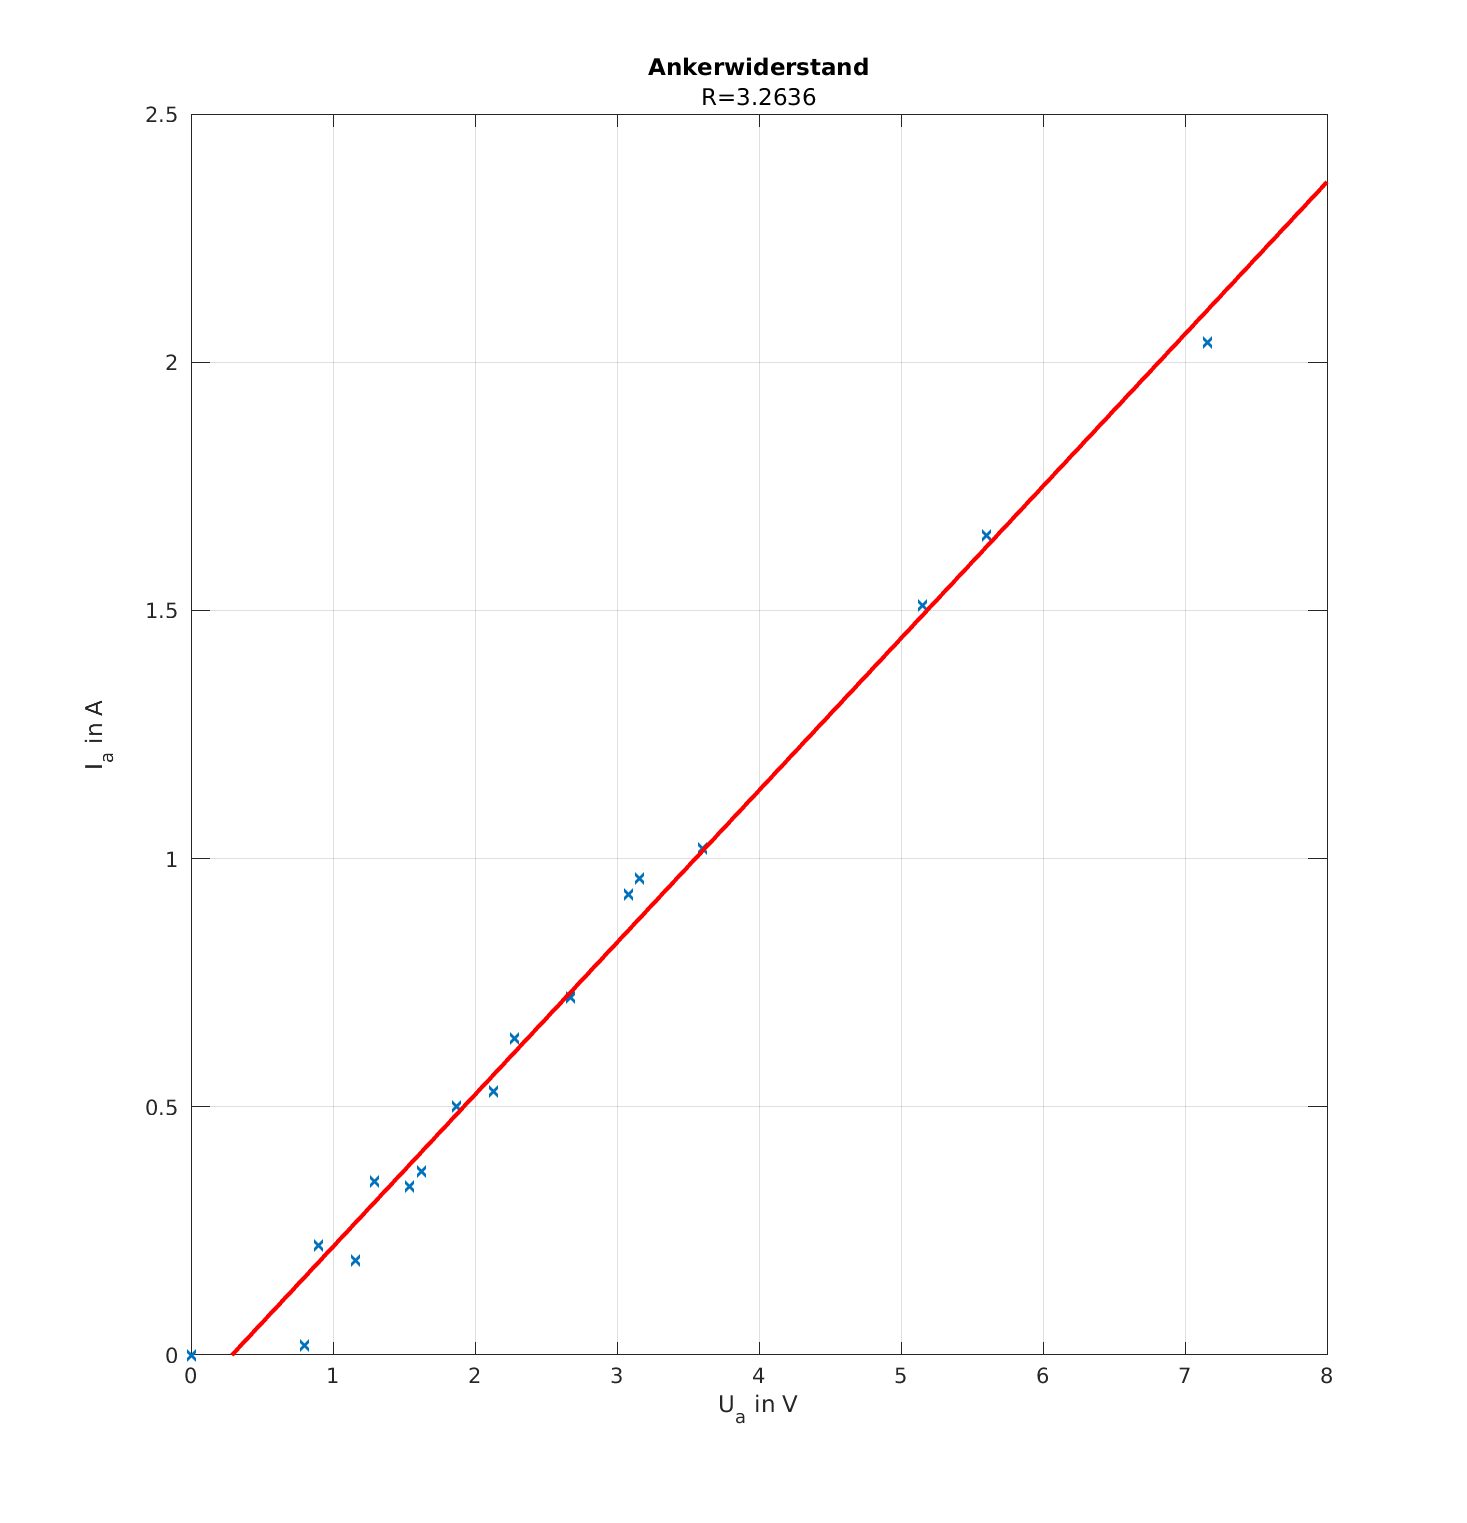
\includegraphics[width=1\textwidth]{as_labor01_2.png}
 \caption{Plot der Aufgabe 2}
 \label{fig:PlotAufgabe2}
\end{figure}
\subsubsection{Messung des Stillstandsdrehmomentes}

Im dritten Versuch soll die Konstante $k_e$ bestimmt werden. Diese
beschreibt als Proportionalfaktor den Zusammengang zwischen der
induzierten Spannung $U_i$ und der Winkelgeschwindigkeit $\omega$.

\begin{equation} \label{eq131}
    \begin{split}
        u_i(t)=k_e \cdot \omega (t)
    \end{split}
\end{equation}

Gegeben sind in dieser Aufgabe sind die Messwerte in einer Matrix. Diese
enthält die Spannungswerten von $U_a=U_i$, welche mit einem Multimeter
gemessen worden sind und den Inkrementen pro $\mathrm{ms}$ $Y$, ermittelt
durch einen Inkrementalgeber und einen Mikrocontroller.

Um $k_e$ zu bestimmen wird neben der direkt gegebenen Spannung $U_a$ auch
die Winkelgeschwindigkeit $\omega$ benötigt. Diese ist das Produkt aus
$2\pi$ und der Drehzahl $n$. Während die Winkelgeschwindigkeit angibt wie
schnell sich ein Winkel mit der Zeit um eine Achse ändert, gibt die Drehzahl
die Anzahl der Umdrehungen in einer Zeitspanne an.

\begin{equation} \label{eq132}
    \begin{split}
        k_e = \frac{U_a}{\omega}= \frac{U_a}{2 \pi n}
    \end{split}
\end{equation}

Die gemessen Inkremente pro Zeit müssen daher umgerechnet werden. Diese
wurden mit dem C167 Mikrocontroller mit einer Abtastzeit $T=1\mathrm{ms}$
aufgenommen. Der Inkrementalgeber besitzt 500 Inkremente pro Umdrehung.
Durch eine Vierfachauswertung ergeben sich $P_z=\frac{2000}{2\pi} \mathrm{\frac{INK}{rad}}$.
Dadurch ergibt sich folgender Umrechnungsfaktor $\lambda$.

\begin{equation} \label{eq133}
    \begin{split}
        \lambda = \frac{1000}{P_z} \mathrm{\frac{ms}{s} \frac{rad}{INK}}
    \end{split}
\end{equation}

Über diesen Faktor lässt sich die Drehzahl bestimmen, damit die
Winkelgeschwindigkeit und abschließend auch $k_e$.

\begin{equation} \label{eq133}
    \begin{split}
        n &= \lambda \cdot Y \qquad \text{in} \mathrm{\frac{rad}{s}}\\
        \omega &= 2 \pi \lambda \cdot Y \qquad \text{in} \mathrm{\frac{rad}{s}}\\
        k_e &= \frac{U_a}{2 \pi \lambda \cdot Y}  \qquad \text{in} \mathrm{\frac{Vs}{rad}}
    \end{split}
\end{equation}

Dadurch berechnet sich $ke$ nach über das Reziproke der Steigung der Funktion
multipliziert mit dem Faktor $\lambda$.

\begin{equation} \label{eq134}
    \begin{split}
    k_e = \frac{1}{m \cdot \lambda} \simeq 0.0235 \mathrm{\frac{Vs}{rad}}
    \end{split}
\end{equation}

\begin{figure}[H]
 \centering
 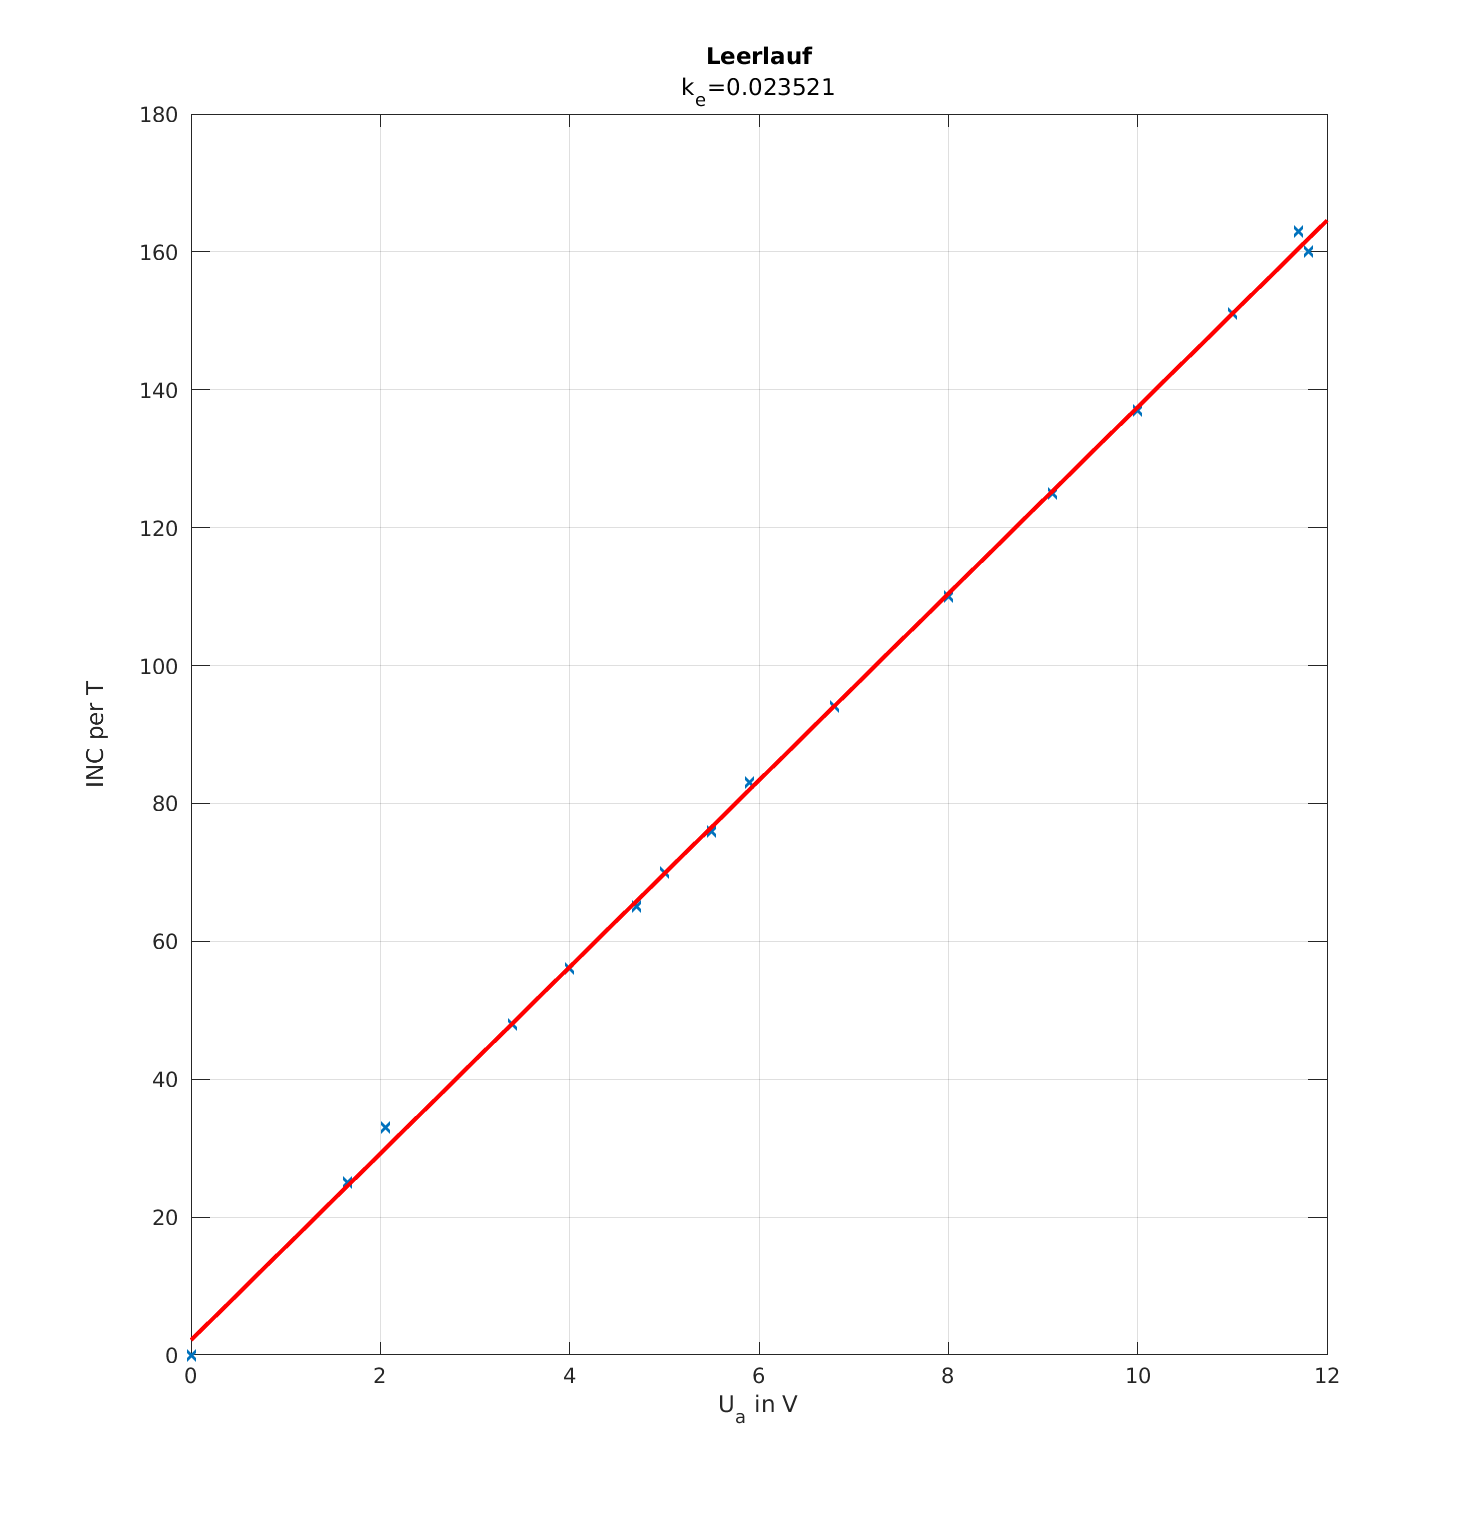
\includegraphics[width=1\textwidth]{as_labor01_3.png}
 \caption{Plot der Aufgabe 3}
 \label{fig:PlotAufgabe3}
\end{figure}
\subsubsection{Messung der Kennlinie des Verstärkers}

In der letzten Messung soll die Kennlinie des Messverstärkers ermittelt
werden und damit der Verstärkungsfaktor $A$ bestimmt werden. Dafür liegt
eine Matrix mit den Eingangsspannungen $U_e$ und den Ausgangspannungen
$U_a$ vor. Da der Verstärker ausgangsseitig bei etwa $+13.75\mathrm{V}$
und $-13.06\mathrm{V}$ in Sättigung geht, werden die jeweils ersten beiden
und die letzten beiden Messwerte für die Berechnung der Funktion nicht
betrachtet.

Der Verstärkungsfaktor $A$ ist der Quotient aus Ausgangs- und Eingangsspannung
und somit die Steigung der ermittelten Funktion.

\begin{equation} \label{eq141}
    \begin{split}
        A=\frac{U_a}{U_e}\simeq2 \mathrm{V}
    \end{split}
\end{equation}

\begin{figure}[H]
 \centering
 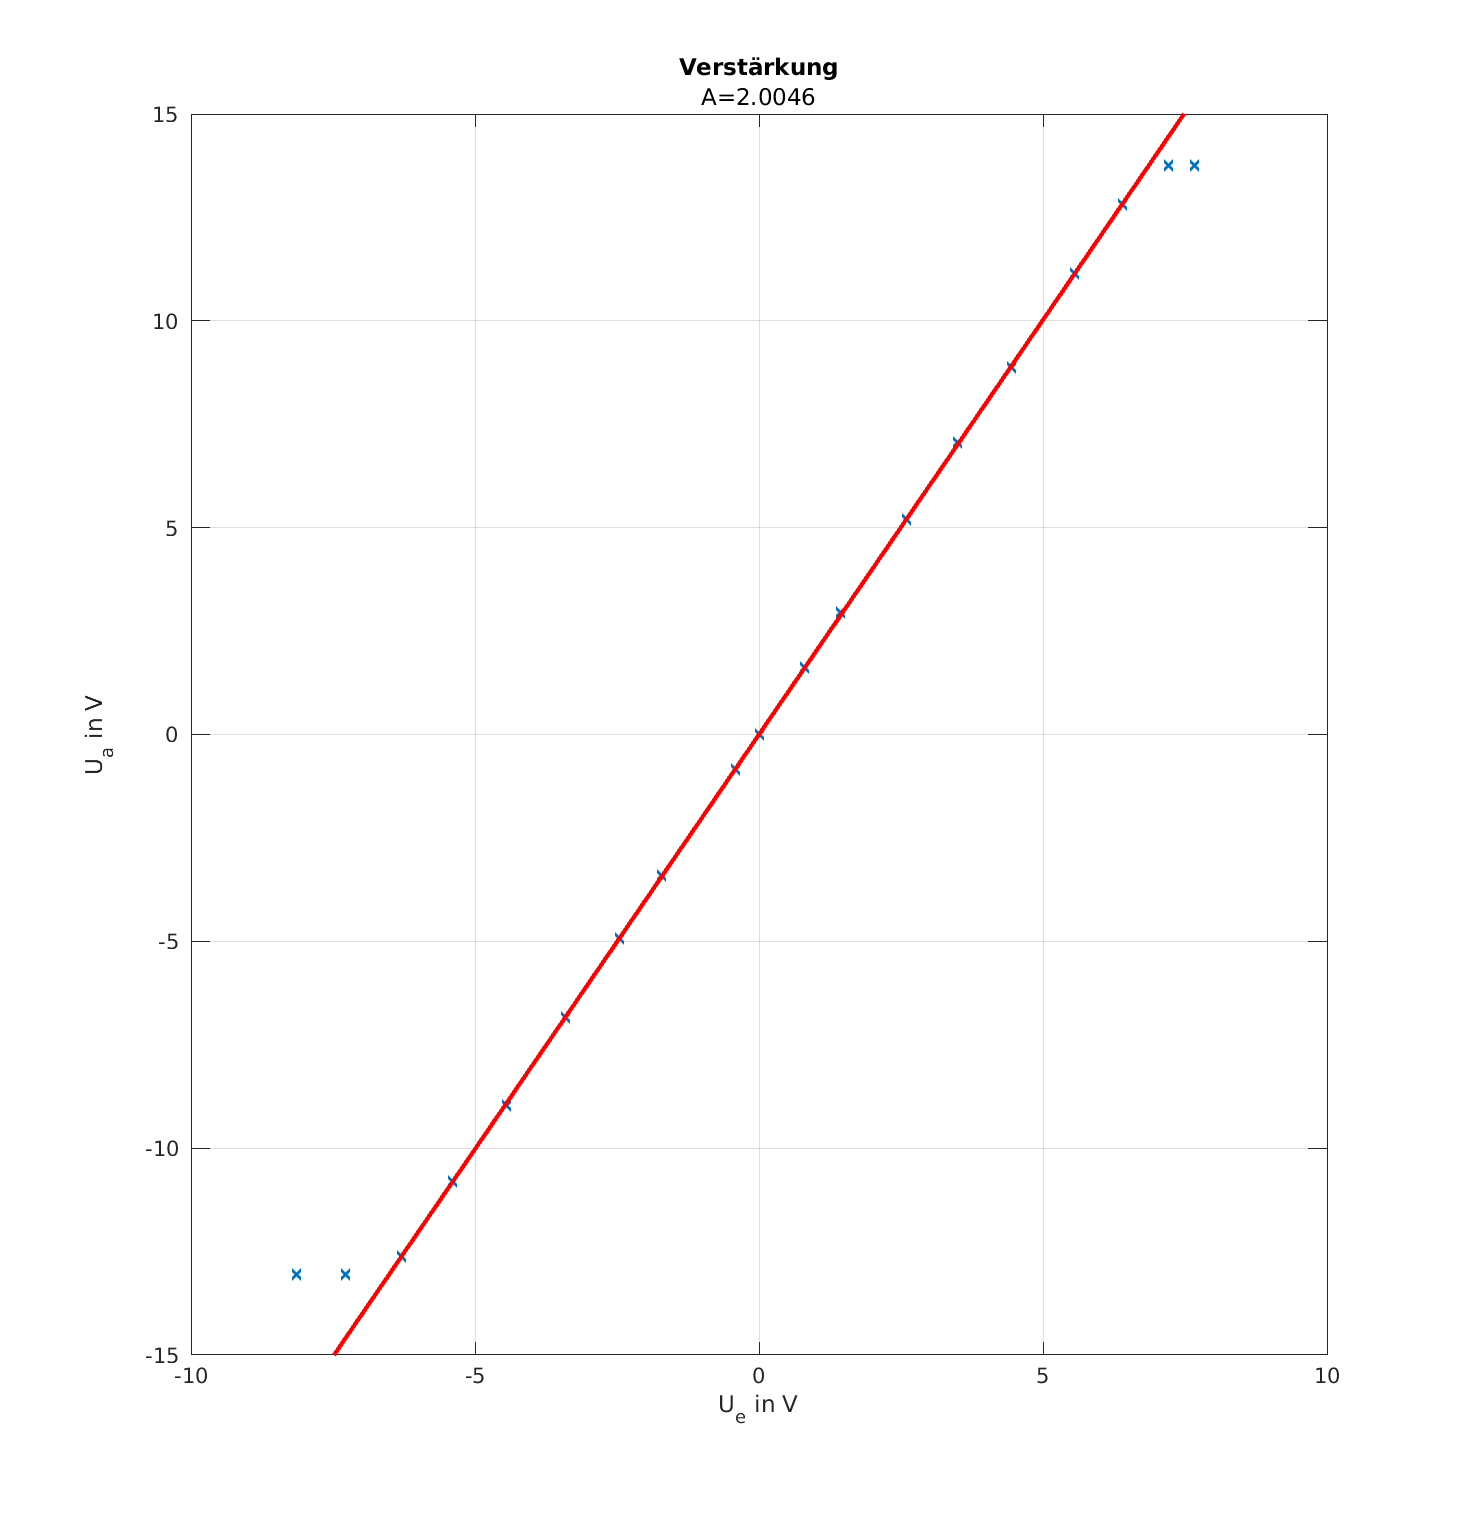
\includegraphics[width=1\textwidth]{as_labor01_4.png}
 \caption{Plot der Aufgabe 4}
 \label{fig:PlotAufgabe4}
\end{figure}
%\subsection{Zusammenfassung}
\subsection{Anhang}

\subsubsection{Aufgabenbeschreibung}
\begin{figure}[H]
    \centering
    \includegraphics[page=3, width=0.8\textwidth]{../Aufgabenstellung.pdf}
    %\caption{Aufbau der CBM-Toolchain}
    \label{fig:Aufgabenstellung A1}
\end{figure}

\begin{figure}[H]
    \centering
    \includegraphics[page=4, width=0.8\textwidth]{../Aufgabenstellung.pdf}
    %\caption{Aufbau der CBM-Toolchain}
    \label{fig:Aufgabenstellung A1}
\end{figure}

\subsubsection{Matlab Code}
\lstinputlisting[language=Matlab]{matlab/as_labor01_1.m}
\lstinputlisting[language=Matlab]{matlab/as_labor01_2.m}
\lstinputlisting[language=Matlab]{matlab/as_labor01_3.m}
\lstinputlisting[language=Matlab]{matlab/as_labor01_4.m}

%\subsubsection{Messwerte}



\end{document}

\section{Labor 2}

\subsection{Einleitung und Ziel}

Im 2. Labor im Modul Aktorik und Sensorik soll die Ankerinduktiviät $L$
und die Reibungskonstante $c_r$ eines Gleichstrommotors bestimmt werden.

%\subsection{Grundlagen und Theorie}
\subsection{Aufgabenstellung und Versuch}

\subsubsection{Bestimmung der Ankerinduktivität}

Um die Ankeridnuktivität zu bestimmen, muss der Motor gebremst sein,
damit die induzierte Gegenspannung $U_{ind} = 0$ ist. Dann ergibt sich
folgendes Schaltbild.


\begin{figure}[H]
    \centering
    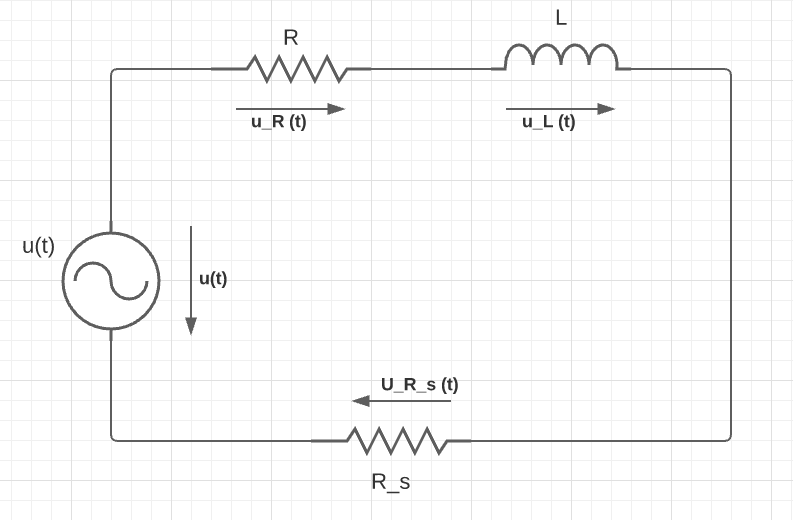
\includegraphics[width=1\textwidth]{schaltplan.png}
    \caption{Mess-Schaltung Ankerinduktivität}
    \label{fig:PlotAufgabe1}
   \end{figure}

Diese Schaltung kann durch folgende Maschengleichung beschrieben werden.

\begin{equation} \label{eq211}
    \begin{split}
        u(t)&=u_R(t) + u_L(t)\\
        u(t)&=R \cdot i(t) + L \frac{d i(t)}{dt}\\
        u(t)&= (R+R_s) \cdot i(t) + L \frac{d i(t)}{dt}
    \end{split}
\end{equation}

Die Idee zur Bestimmung der Induktivität ist nun folgende. Die Schaltung
wird mit einer sinusförmigen Wechselspannung betrieben. Über die
Phasenverschiebung der Eingangsspannung und des Stromes kann die Induktivität
bestimmt werden.

\begin{equation} \label{eq212}
    \begin{split}
        \underline{U} = A \cdot e^{\jmath 0}\\
        \underline{I} = B \cdot e^{\jmath \varphi}
    \end{split}
\end{equation}

Der Strom $i(t)$ wird indirekt über den Messwiderstand $R_s= 1\Omega$
bestimmt, da folgendes gilt.

\begin{equation} \label{eq213}
    \begin{split}
        i(t)=\frac{u_{Rs}(t)}{R_s} = u_{Rs}(t)
    \end{split}
\end{equation}

Der Phasenwinkel kann über die Impedanz $\underline{Z}$ berechnet werden.

\begin{equation} \label{eq214}
    \begin{split}
        \underline{Z} &= (R + R_s) + \jmath \omega L\\
        \varphi\{\underline{Z} \} &= \arctan \left( \frac{\omega L}{ R + R_s} \right)
    \end{split}
\end{equation}

Da nicht der Phasenwinkel $\varphi$ sondern die Phasenverschiebung $\Delta t$ gemessen
wird, muss dieser noch umgerechnet werden.

\begin{equation} \label{eq215}
    \begin{split}
        \varphi &= \frac{\Delta t}{T} \cdot 2 \pi \\
        \varphi &=  \omega \Delta t = 2 \pi f \Delta t
    \end{split}
\end{equation}

Nun lässt sich die Induktivität $L$ folgendermaßen berechnen.

\begin{equation} \label{eq216}
    \begin{split}
        L = \frac{(R+R_s) }{2 \pi f} \cdot \tan(2 \pi f \Delta t)
    \end{split}
\end{equation}

Da in der Messung die Phasenverschiebung $\Delta t$ in Abhängigkeit
von der Frequenz $f$ gemessen worden ist, ergibt sich die Funktion $f_1(f)$.

\begin{equation} \label{eq217}
    \begin{split}
       \Delta t = f_1(f) = \frac{1}{2 \pi f} \arctan \left( \frac{2 \pi L}{R + R_s} f \right)
    \end{split}
\end{equation}

Um diese Funktion zu Linearisieren muss diese noch umgestellt werden.

\begin{equation} \label{eq218}
    \begin{split}
       \tan(2 \pi f \Delta t) = f_2(f) = \frac{2 \pi L}{R + R_s} f
    \end{split}
\end{equation}

Nun kann mittels der linearen Regression aus den beiden Vektoren die Steigung
$m$ bestimmt werden, aus der sich die Induktivität $L$ berechnen lässt.

\begin{equation} \label{eq219}
    \begin{split}
       m &=  \frac{2 \pi L}{R + R_s}\\
       L &= \frac{m \cdot (R+R_s)}{2 \pi} \simeq 175.462 \mathrm{\mu H}
    \end{split}
\end{equation}


\begin{figure}[H]
 \centering
    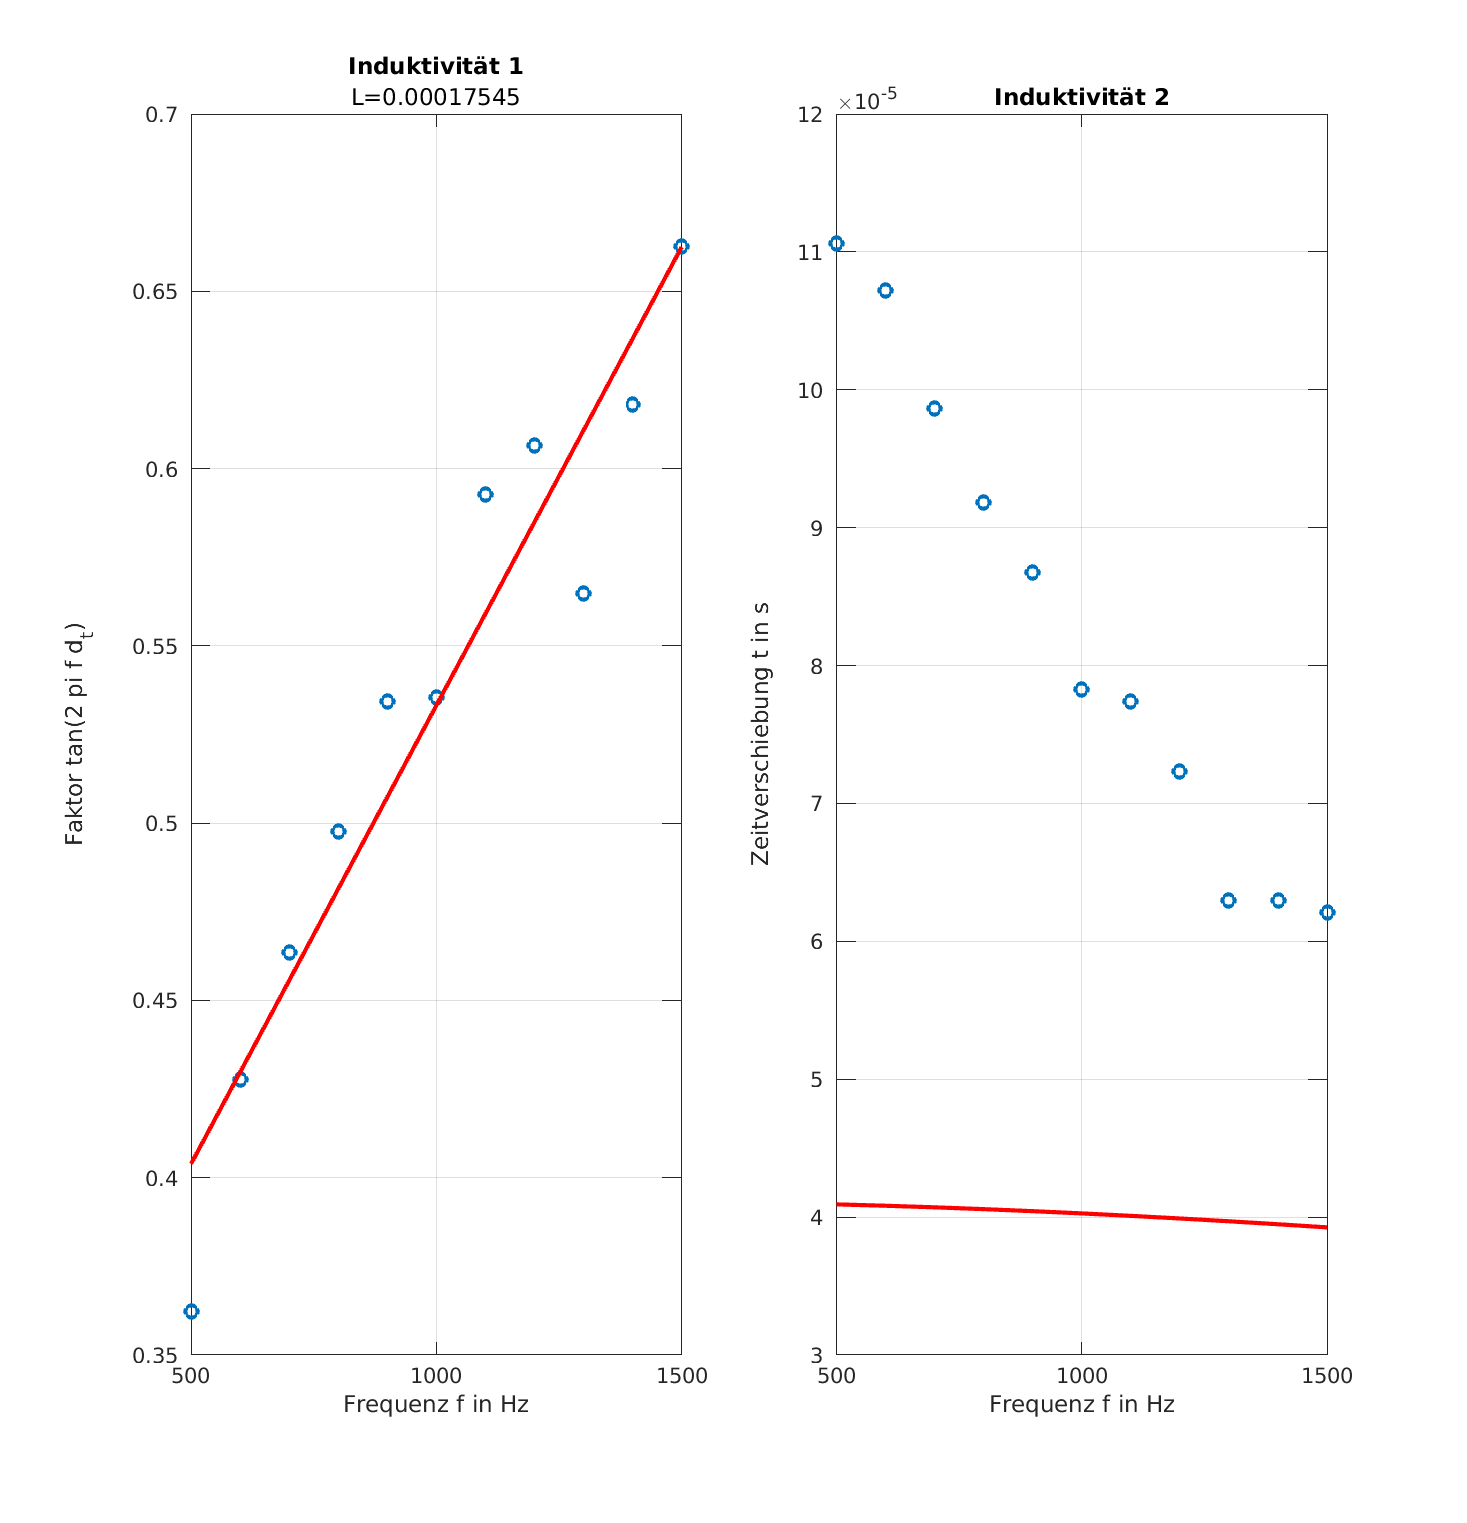
\includegraphics[width=1\textwidth]{as_labor02_1.png}
 \caption{Plot der Aufgabe 1}
 \label{fig:PlotAufgabe1}
\end{figure}
\subsubsection{Bestimmung der Reibungskonstanten}

Die Reibungskonstante kann über folgende DGL berechnet werden.
Die Summe der Drehmomente ergibt sich aus dem Drehmoment $M_m$
abzüglich des Reibungsdrehmoments $M_R$ und des Lastdrehmoments.
Diese sind gleich der zeitlichen Änderung der Winkelgeschwindikeit 
$\frac{d \omega}{dt}$ multipliziert mit dem Trägheitsmoment $J$.

\begin{equation} \label{eq221}
    \begin{split}
        J \frac{d \omega}{d t} &= \sum M = M_m - M_R - M_L \\
        J \frac{d \omega}{d t} &= \sum M = k_m \cdot i(t) - c_r \omega (t) - M_L 
    \end{split}
\end{equation}

Um die Reibungskonstante $c_r$ nun zu bestimmen, ist es günstig das
System im Leerlauf zu betrachten, da $M_L=0$ und nach Abklingen des
Einschaltvorgangs $\frac{d\omega}{dt} =0$. Aus der DGL ergibt sich
folgende einfache Gleichung.

\begin{equation} \label{eq222}
    \begin{split}
        0 & = k_m \cdot i(t) - c_r \omega (t)
    \end{split}
\end{equation}

Daraus ergibt sich folgende Funktion.

\begin{equation} \label{eq222}
    \begin{split}
        \omega = f_3(i) = \frac{k_m}{c_r} i
    \end{split}
\end{equation}

Nun kann mittels der linearen Regression aus den beiden Vektoren die Steigung
$m$ bestimmt werden, aus der sich die Reibungskonstante $c_r$ berechnen lässt.

\begin{equation} \label{eq218}
    \begin{split}
       m &=  \frac{k_m}{c_r}\\
       c_r &= \frac{k_m}{m} \simeq 3,24 \cdot 10^{-9} \mathrm{\frac{Nm s}{rad}}
    \end{split}
\end{equation}

\begin{figure}[H]
 \centering
    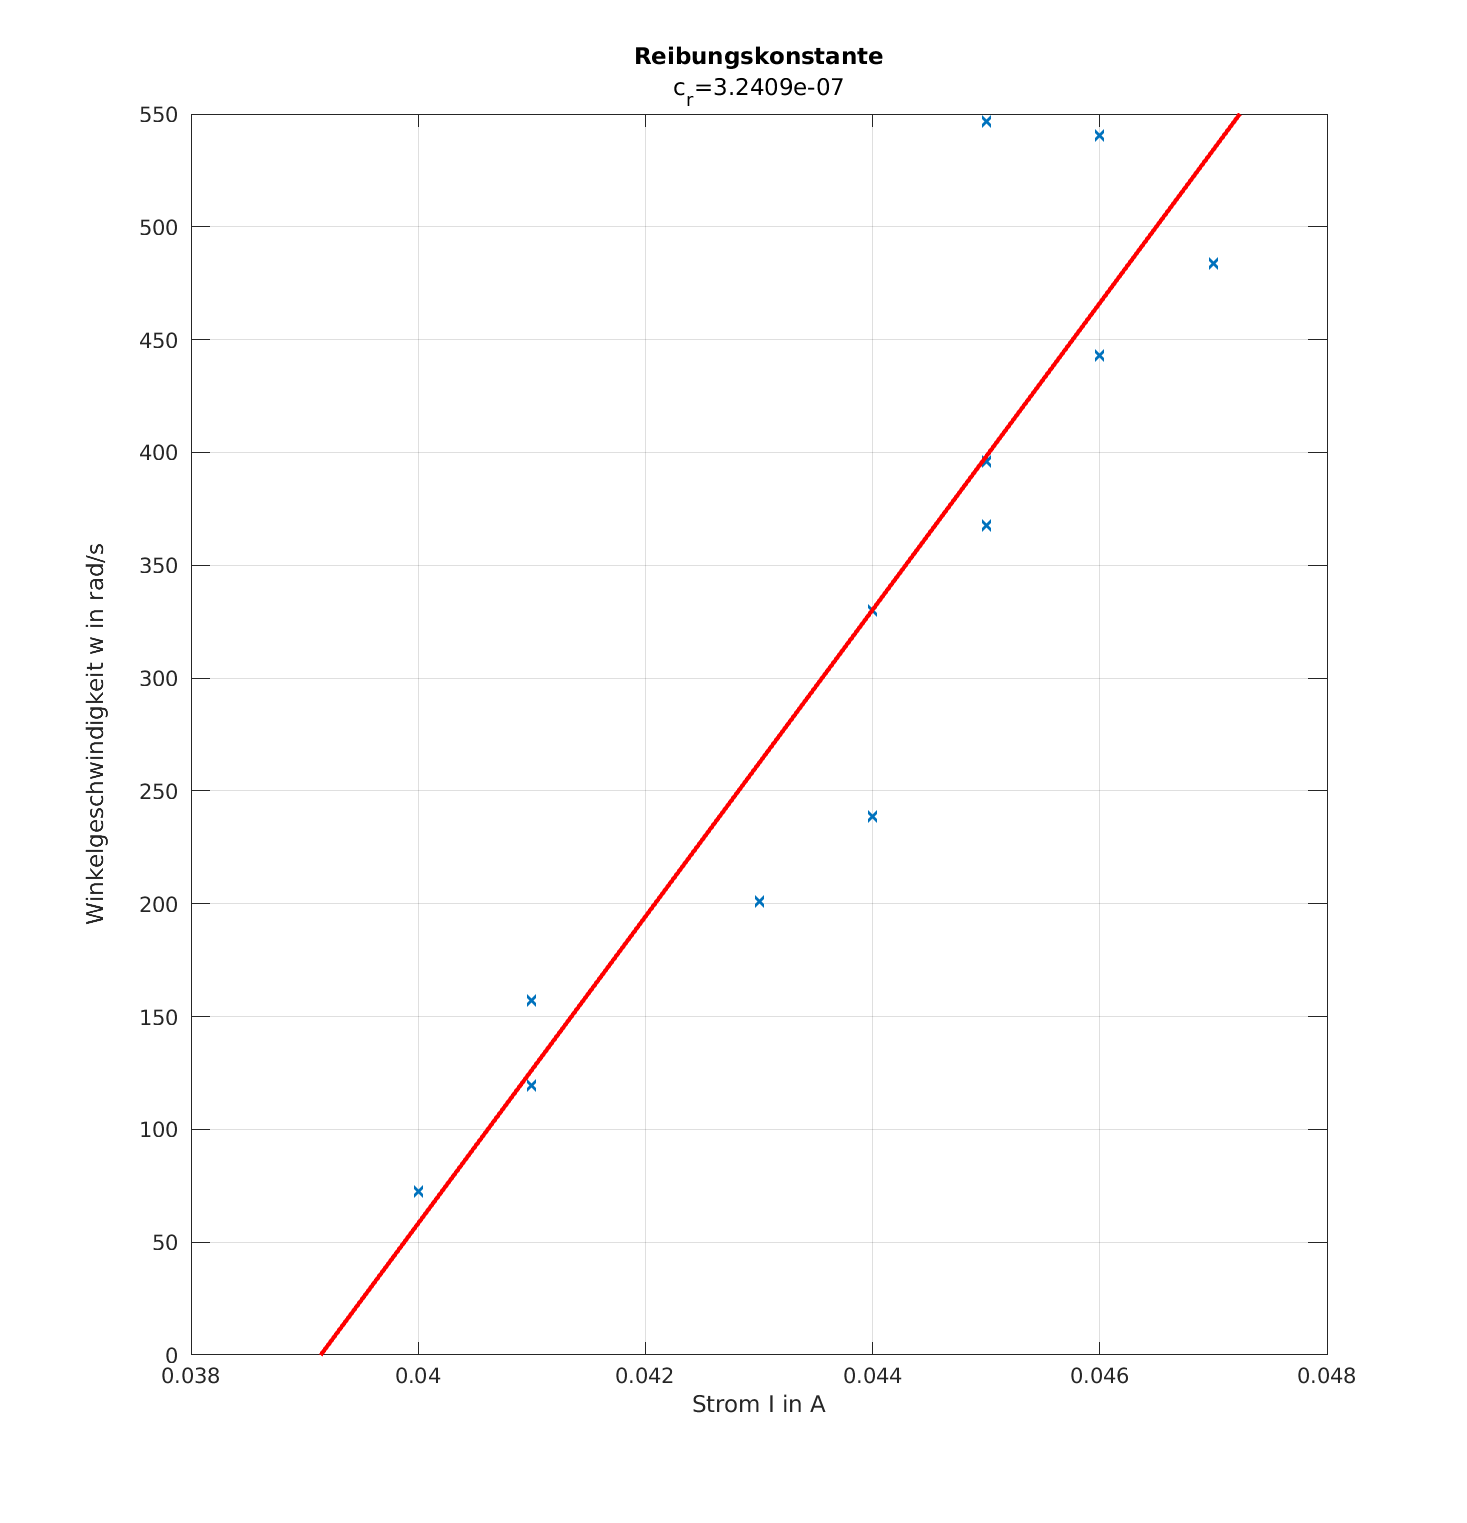
\includegraphics[width=1\textwidth]{as_labor02_2.png}
 \caption{Plot der Aufgabe 1}
 \label{fig:PlotAufgabe1}
\end{figure}
\subsection{Zusammenfassung}

Mittels der Messwerte sind wir auf folgende Werte für die Ankerinduktivität $L$
und die Reibungskonstante $c_r$ gekommen.

\begin{equation} \label{eq241}
    \begin{split}
       L &=  175.462 \mathrm{\mu H}\\
       c_r &= 3,24 \cdot 10^{-9} \mathrm{\frac{Nm s}{rad}}
    \end{split}
\end{equation}

Die Berechnung der Reibungskonstante stellte uns vor keine Herausforderung
und ist sowohl Einheitenmäßig als auch Dimensionsmäßig nachvollziehbar.\\

Die Bestimmung der Ankerinduktivität stellte uns allerdings vor die
Herausforderung das System zu liniearisieren (Abbildung 2: Induktivität 1).
Nach der Liniearisierung der Funktion und anschließender Regression haben wir
den errechneten Wert der Induktivität wieder in die Ursprungsfunktion eingesetzt
(Abbildung 2: Induktivität 2). Hier ist zu erkennen, dass die ermittelte Gerade
sich nur bedingt in der Nähe der Messpunkte befindet. Wir vermuten, dass entweder
eine Ungenauigkeit in unseren Modell vorhanden ist oder es ist einen vielleicht
sogar frequenzabhängigen Offset in den Messdaten gibt. Um dieses Verhalten genauer
zu untersuchen, haben wir die Funktion und die Messdaten \href{https://www.desmos.com/calculator/2je7stqm76}{interaktiv in Desmos}
erstellt.\\

Wir konnten diese Diskrepanz leider nicht abschließend klären, sind aber zum Entschluss
gekommen das unser Ergebnis von $175.462 \mathrm{\mu H}$ ausreichend genau und auch realistisch ist.
\subsection{Anhang}

\subsubsection{Aufgabenbeschreibung}
\begin{figure}[H]
    \centering
    \includegraphics[page=5, width=0.8\textwidth]{../Aufgabenstellung.pdf}
    %\caption{caption}
    \label{fig:Aufgabenstellung Labor 2.1}
\end{figure}

\begin{figure}[H]
    \centering
    \includegraphics[page=6, width=0.8\textwidth]{../Aufgabenstellung.pdf}
    \label{fig:Aufgabenstellung Labor 2.2}
\end{figure}

\subsubsection{Matlab Code}
\lstinputlisting[language=Matlab]{matlab/as_labor02_1.m}
\lstinputlisting[language=Matlab]{matlab/as_labor02_2.m}

%\subsubsection{Messwerte}

% % !TEX root = ./main.tex

\documentclass[a4paper, 12pt, halfparskip]{article}
\usepackage[utf8]{inputenc}
\usepackage[ngerman]{babel}
\usepackage{pdfpages}
\usepackage{graphicx}
\usepackage{amsmath}

\graphicspath{ {./img/} }
\usepackage{hyperref}
\usepackage{lipsum}
\usepackage{float}
\usepackage{listings}
\usepackage[left=2.7cm, right=2.7cm, top=2.7cm, bottom=2.7cm]{geometry}

\usepackage{xcolor}

\definecolor{codegreen}{rgb}{0,0.6,0}
\definecolor{codegray}{rgb}{0.5,0.5,0.5}
\definecolor{codepurple}{rgb}{0.58,0,0.82}
\definecolor{backcolour}{rgb}{0.95,0.95,0.92}

\setlength{\parindent}{0pt}

\lstdefinestyle{mystyle}{
    backgroundcolor=\color{backcolour},   
    commentstyle=\color{codegreen},
    keywordstyle=\color{magenta},
    numberstyle=\tiny\color{codegray},
    stringstyle=\color{codepurple},
    basicstyle=\ttfamily\footnotesize,
    breakatwhitespace=false,         
    breaklines=true,                 
    captionpos=b,                    
    keepspaces=true,                 
    numbers=left,                    
    numbersep=5pt,                  
    showspaces=false,                
    showstringspaces=false,
    showtabs=false,                  
    tabsize=2
}

\lstset{style=mystyle}
\lstset{literate=%
{Ö}{{\"O}}1
{Ä}{{\"A}}1
{Ü}{{\"U}}1
{ß}{{\ss}}2
{ü}{{\"u}}1
{ä}{{\"a}}1
{ö}{{\"o}}1
}

\newcommand{\nr}{1}


\title{Aktorik Sensorik \\ Labor 3}
\author{Anton Kress (S872899), Jan Abel (S876662)}
\date{Dezember 2020}

\begin{document}

\maketitle

\newpage
\tableofcontents 
\section{Labor 3}

\subsection{Einleitung und Ziel}

Im 3. Labor des Moduls Aktorik und Sensorik soll ein mathematische Modell
eines Gleichstrommotors aufgestellt und in Simulink umgesetzt werden.\\

Die dafür nötigen Konstanten (u.a Ankerwiderstand, Induktivität, etc.)
sind in den beiden vergangenen Versuchen bereits bestimmt worden.
Um das Trägheits-moment $J$ -- die einzige fehlende Konstante im Modell --
zu bestimmen, wird das Modell mit einer Messung am realen System
verglichen. In dieser Messung wurde ein Spannungs-Sprung auf den Motor
gegeben und der Strom als Sprungantwort aufgenommen.
\subsection{Grundlagen und Theorie}

Das Blocksschaltbild, welches in Simulink umzusetzten ist, resultiert aus
den beiden folgenden DGL.

\begin{equation} \label{eq211}
    \begin{split}
        \dot{i(t)}&=\frac{1}{L} \left[ u(t) - (R + R_s) \cdot i(t) - ke \cdot \omega(t) \right]\\
        \dot{\omega(t)}&=\frac{1}{J} \left[km \cdot i(t) -C_r \omega(t) \right]
    \end{split}
\end{equation}

Die erste Gleichung ergibt sich aus der Maschengleichung des elektrischen Teils.
Der zweite Teil der DGL ist auf die Summation der Drehmomente zurückzuführen.
\subsection{Aufgabenstellung und Versuch}

Aus den bereits aufgestellten DGL-System kann das Blockschaltbild in Simulink
erstellt werden.

\begin{figure}[H]
    \centering
    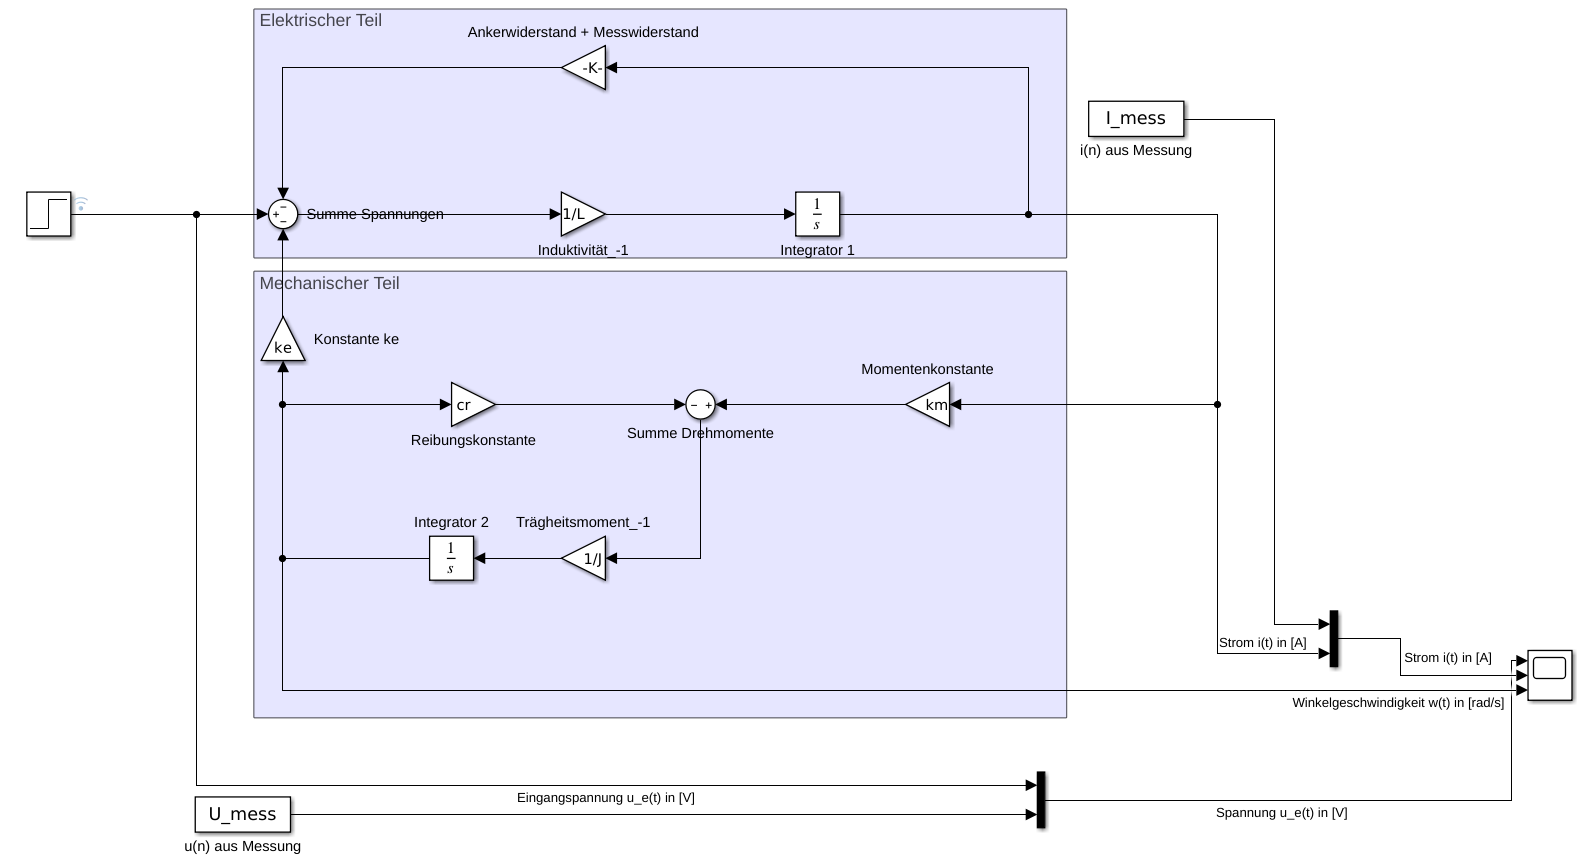
\includegraphics[width=1\textwidth]{sl_modell.png}
    \caption{Blockschaltbild in Simulink}
    \label{fig:Blockschaltbild}
\end{figure}

Als Eingang wurde ein Step-Block benutzt und als Ausgang ein Scope-Block.
Die erste DGL wurden im oberen Teil des Modell realisiert und beschreibt
den elektrischen Teil des Systems. Im unteren wird der mechanische Teil
des Motors modelliert der aus der zweiten DGL hervorgeht.\\

Die schon ermittelten Konstanten des Systems wurden in einem Matlab-File
abgespeichert und werden über dieses auch aufgerufen. Auch die Daten der
Messung des Spungs und der Sprungantwort sind hier zufinden.\\

Um den gemessenen Spung und die Sprungantwort in Simulink anzuzeigen wurde der Block
"From Workspace" benutzt der jeweils den Zeit-Spannungs-Vektor und den Zeit-
Spannungs-Vektor lädt.\\

Der Spung aus dem Modell wurden dem Sprung aus der Messung mit folgenden
Parameter angepasst.\\

\begin{figure}[H]
    \centering    
    \begin{tabular}[h]{l| r}
        Steptime & 0.048s \\
        \hline
        Final Value & 8.2V \\
        \hline
        Sampletime & 0.001s \\
    \end{tabular}
    \caption{Parameter Step Block}
\end{figure}
    

Um das Trägheitsmoment $J$ zu bestimmen, wurde dann $J$ auf den Initialwert
von $10^{-3}\mathrm{Kg \cdot m^2}$ gesetzt. Dieser stammt aus dem Datenblatt
des DCX10L aus der Vorlesung.

Danach haben wir das System für 30 Sekunden simuliert und erhielten folgendes
Ergebnis.

\begin{figure}[H]
    \centering
    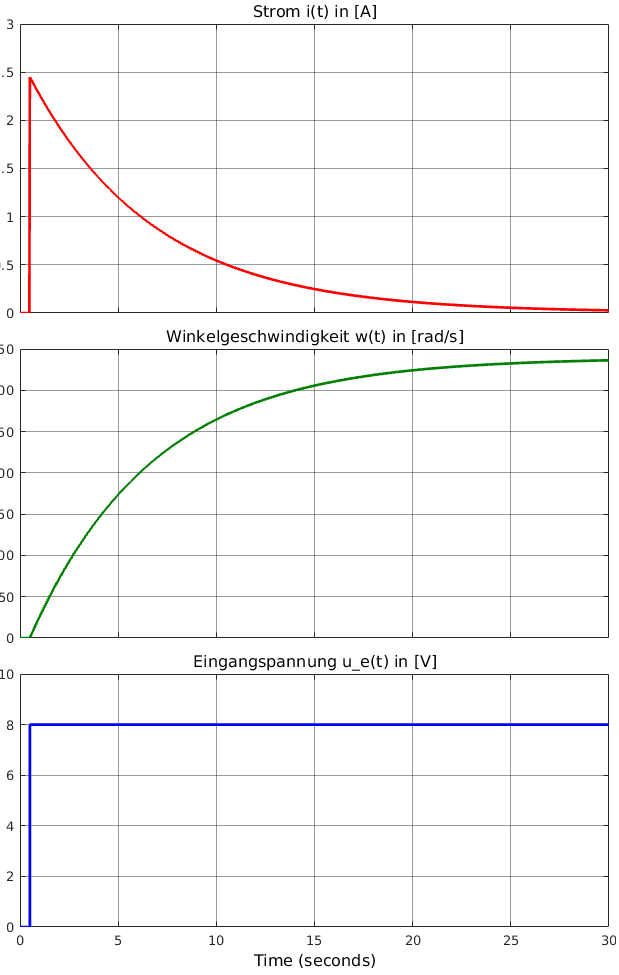
\includegraphics[width=0.75\textwidth]{data_modell.png}
    \caption{Simulation 1}
    \label{fig:Simulation 1}
\end{figure}

Wir haben dann durch manuelles iteratives Anpassen den Wert des Trägheitsmoments
so bestimmt, dass die Funktion des Modells mit den Messdaten übereinstimmt. 

\begin{equation} \label{eq311}
    \begin{split}
        J \simeq 5 \mathrm{\mu Kg \cdot m^2}
    \end{split}
\end{equation}

Anschließend simulierten wir in der Zeit der gegebenen Messdaten  $\Delta T= 0.6s$.
Daraus ergab sich folgendes Ergebnis.

\begin{figure}[H]
    \centering
    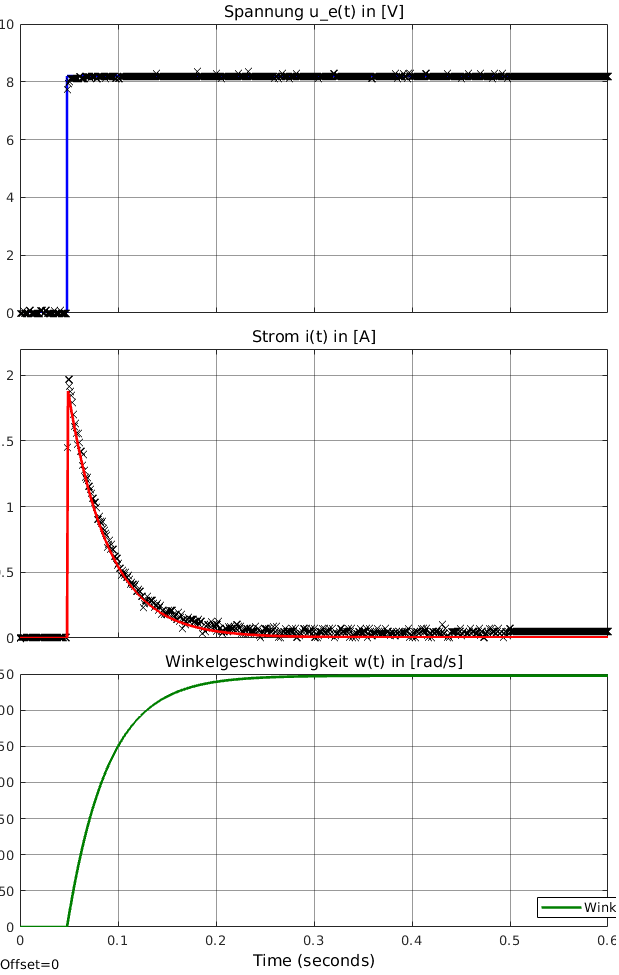
\includegraphics[width=0.75\textwidth]{data_modell_final.png}
    \caption{Simulation 2}
    \label{fig:Simulation 2}
\end{figure}
\subsection{Diskussion und Zusammenfassung}

Der exponentiell fallende Stromverlauf ist ein normales Verhalten des Anlaufstroms eines
Motors. Dies ist daher zu erklären, dass die Schwungmasse an der Welle des Motors aus
der Ruhelage erst auf Nenndrehzahl gebracht werden muss. Dafür ist im Anschaltmoment
eine große Energie nötig, welche über den erhöhten Strom zugeführt wird.\\

Die errechneten Funktionen unseres Modells stimmen nahezu vollständig mit den gemessenen
Daten überein. Sie liegen unter einer maximalen Abweichung von 5\%. Dieses gute Ergebnis
ist auf ein ausreichend gutes Modell und valide Messdaten zurückzuführen.\\
\subsection{Anhang}

\subsubsection{Aufgabenbeschreibung}
\begin{figure}[H]
    \centering
    \includegraphics[page=7, width=0.8\textwidth]{../Aufgabenstellung.pdf}
    %\caption{caption}
    \label{fig:Aufgabenstellung Labor 3}
\end{figure}


\subsubsection{Matlab Code}
\lstinputlisting[language=Matlab]{matlab/as_labor03_const_u_motor_dc.m}

%\subsubsection{Messwerte}

\end{document}

\section{Labor 3}

\subsection{Einleitung und Ziel}

Im 3. Labor des Moduls Aktorik und Sensorik soll ein mathematische Modell
eines Gleichstrommotors aufgestellt und in Simulink umgesetzt werden.\\

Die dafür nötigen Konstanten (u.a Ankerwiderstand, Induktivität, etc.)
sind in den beiden vergangenen Versuchen bereits bestimmt worden.
Um das Trägheits-moment $J$ -- die einzige fehlende Konstante im Modell --
zu bestimmen, wird das Modell mit einer Messung am realen System
verglichen. In dieser Messung wurde ein Spannungs-Sprung auf den Motor
gegeben und der Strom als Sprungantwort aufgenommen.
\subsection{Grundlagen und Theorie}

Das Blocksschaltbild, welches in Simulink umzusetzten ist, resultiert aus
den beiden folgenden DGL.

\begin{equation} \label{eq211}
    \begin{split}
        \dot{i(t)}&=\frac{1}{L} \left[ u(t) - (R + R_s) \cdot i(t) - ke \cdot \omega(t) \right]\\
        \dot{\omega(t)}&=\frac{1}{J} \left[km \cdot i(t) -C_r \omega(t) \right]
    \end{split}
\end{equation}

Die erste Gleichung ergibt sich aus der Maschengleichung des elektrischen Teils.
Der zweite Teil der DGL ist auf die Summation der Drehmomente zurückzuführen.
\subsection{Aufgabenstellung und Versuch}

Aus den bereits aufgestellten DGL-System kann das Blockschaltbild in Simulink
erstellt werden.

\begin{figure}[H]
    \centering
    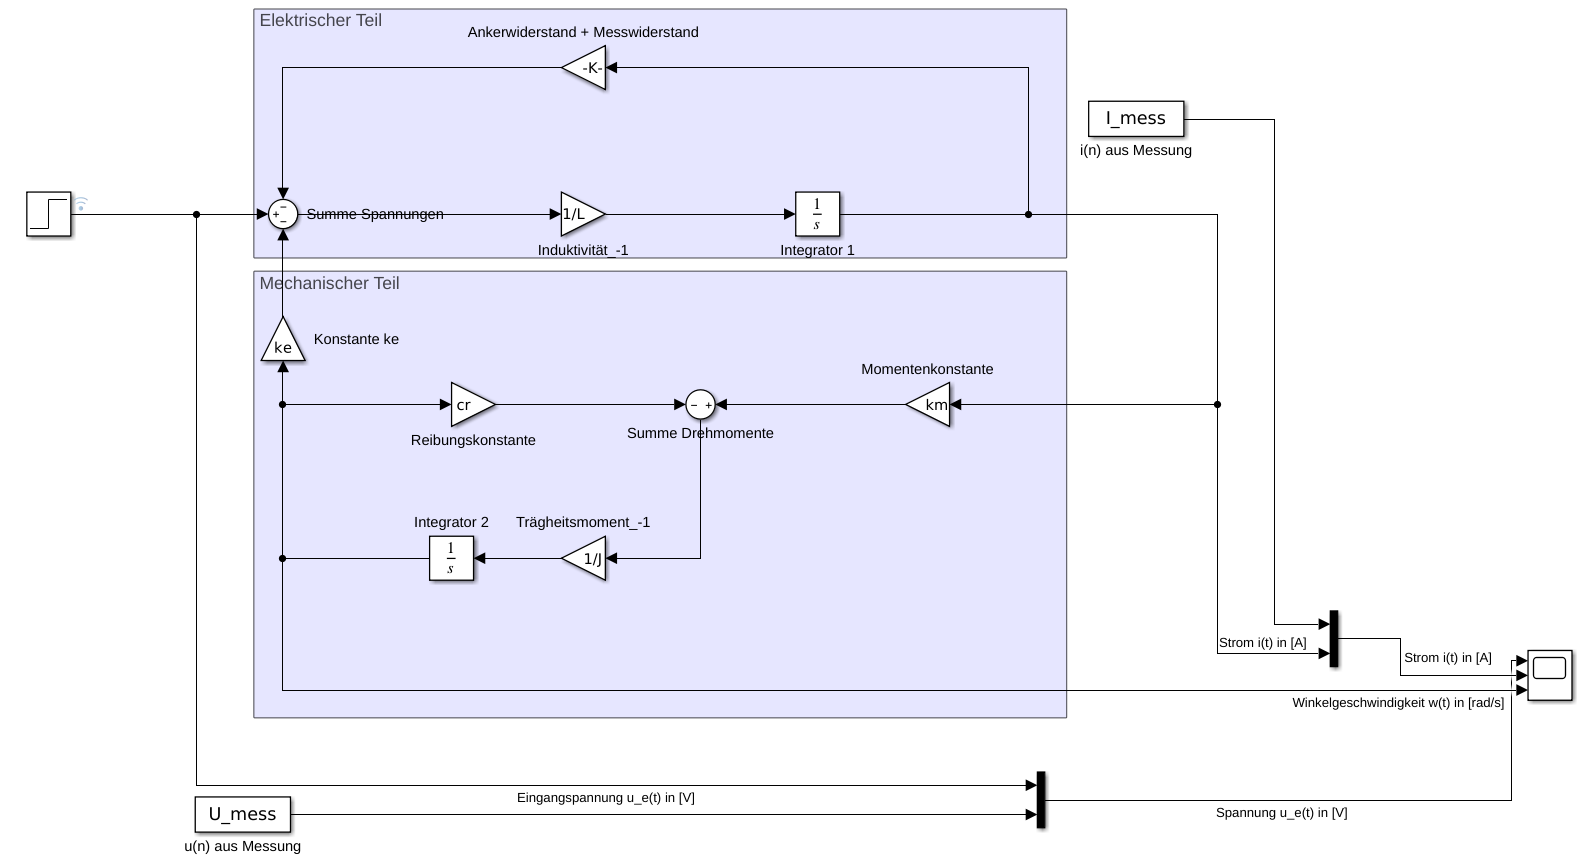
\includegraphics[width=1\textwidth]{sl_modell.png}
    \caption{Blockschaltbild in Simulink}
    \label{fig:Blockschaltbild}
\end{figure}

Als Eingang wurde ein Step-Block benutzt und als Ausgang ein Scope-Block.
Die erste DGL wurden im oberen Teil des Modell realisiert und beschreibt
den elektrischen Teil des Systems. Im unteren wird der mechanische Teil
des Motors modelliert der aus der zweiten DGL hervorgeht.\\

Die schon ermittelten Konstanten des Systems wurden in einem Matlab-File
abgespeichert und werden über dieses auch aufgerufen. Auch die Daten der
Messung des Spungs und der Sprungantwort sind hier zufinden.\\

Um den gemessenen Spung und die Sprungantwort in Simulink anzuzeigen wurde der Block
"From Workspace" benutzt der jeweils den Zeit-Spannungs-Vektor und den Zeit-
Spannungs-Vektor lädt.\\

Der Spung aus dem Modell wurden dem Sprung aus der Messung mit folgenden
Parameter angepasst.\\

\begin{figure}[H]
    \centering    
    \begin{tabular}[h]{l| r}
        Steptime & 0.048s \\
        \hline
        Final Value & 8.2V \\
        \hline
        Sampletime & 0.001s \\
    \end{tabular}
    \caption{Parameter Step Block}
\end{figure}
    

Um das Trägheitsmoment $J$ zu bestimmen, wurde dann $J$ auf den Initialwert
von $10^{-3}\mathrm{Kg \cdot m^2}$ gesetzt. Dieser stammt aus dem Datenblatt
des DCX10L aus der Vorlesung.

Danach haben wir das System für 30 Sekunden simuliert und erhielten folgendes
Ergebnis.

\begin{figure}[H]
    \centering
    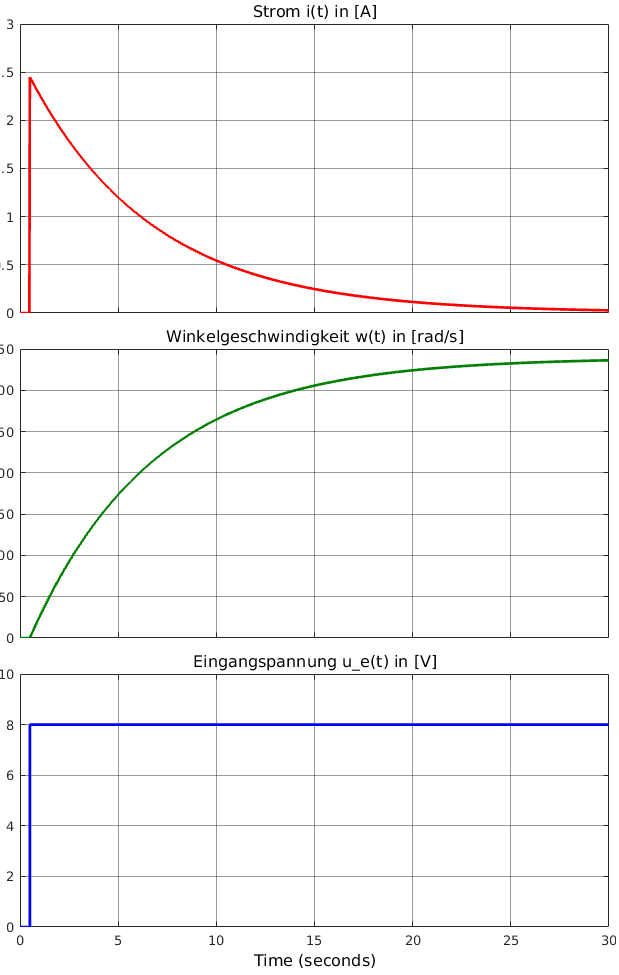
\includegraphics[width=0.75\textwidth]{data_modell.png}
    \caption{Simulation 1}
    \label{fig:Simulation 1}
\end{figure}

Wir haben dann durch manuelles iteratives Anpassen den Wert des Trägheitsmoments
so bestimmt, dass die Funktion des Modells mit den Messdaten übereinstimmt. 

\begin{equation} \label{eq311}
    \begin{split}
        J \simeq 5 \mathrm{\mu Kg \cdot m^2}
    \end{split}
\end{equation}

Anschließend simulierten wir in der Zeit der gegebenen Messdaten  $\Delta T= 0.6s$.
Daraus ergab sich folgendes Ergebnis.

\begin{figure}[H]
    \centering
    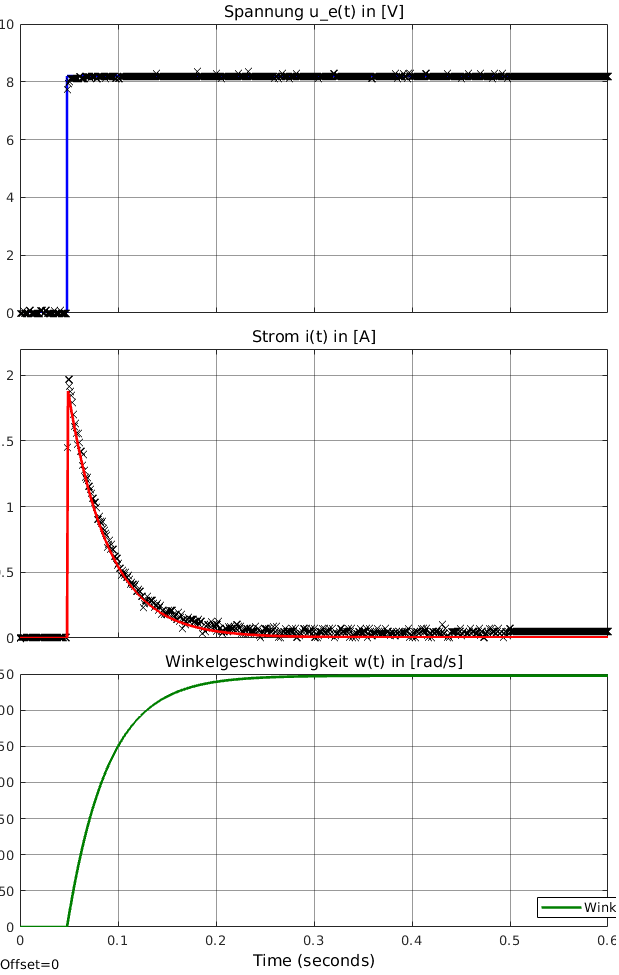
\includegraphics[width=0.75\textwidth]{data_modell_final.png}
    \caption{Simulation 2}
    \label{fig:Simulation 2}
\end{figure}
\subsection{Diskussion und Zusammenfassung}

Der exponentiell fallende Stromverlauf ist ein normales Verhalten des Anlaufstroms eines
Motors. Dies ist daher zu erklären, dass die Schwungmasse an der Welle des Motors aus
der Ruhelage erst auf Nenndrehzahl gebracht werden muss. Dafür ist im Anschaltmoment
eine große Energie nötig, welche über den erhöhten Strom zugeführt wird.\\

Die errechneten Funktionen unseres Modells stimmen nahezu vollständig mit den gemessenen
Daten überein. Sie liegen unter einer maximalen Abweichung von 5\%. Dieses gute Ergebnis
ist auf ein ausreichend gutes Modell und valide Messdaten zurückzuführen.\\
\subsection{Anhang}

\subsubsection{Aufgabenbeschreibung}
\begin{figure}[H]
    \centering
    \includegraphics[page=7, width=0.8\textwidth]{../Aufgabenstellung.pdf}
    %\caption{caption}
    \label{fig:Aufgabenstellung Labor 3}
\end{figure}


\subsubsection{Matlab Code}
\lstinputlisting[language=Matlab]{matlab/as_labor03_const_u_motor_dc.m}

%\subsubsection{Messwerte}

% % !TEX root = ./main.tex

\documentclass{article}
\usepackage[utf8]{inputenc}
\usepackage[ngerman]{babel}
\usepackage{pdfpages}
\usepackage{graphicx}
\usepackage{amsmath}

\graphicspath{ {./img/} }
\usepackage{hyperref}
\usepackage{lipsum}
\usepackage{float}
\usepackage{listings}

\usepackage{xcolor}

\definecolor{codegreen}{rgb}{0,0.6,0}
\definecolor{codegray}{rgb}{0.5,0.5,0.5}
\definecolor{codepurple}{rgb}{0.58,0,0.82}
\definecolor{backcolour}{rgb}{0.95,0.95,0.92}

\lstdefinestyle{mystyle}{
    backgroundcolor=\color{backcolour},   
    commentstyle=\color{codegreen},
    keywordstyle=\color{magenta},
    numberstyle=\tiny\color{codegray},
    stringstyle=\color{codepurple},
    basicstyle=\ttfamily\footnotesize,
    breakatwhitespace=false,         
    breaklines=true,                 
    captionpos=b,                    
    keepspaces=true,                 
    numbers=left,                    
    numbersep=5pt,                  
    showspaces=false,                
    showstringspaces=false,
    showtabs=false,                  
    tabsize=2
}

\lstset{style=mystyle}
\lstset{literate=%
{Ö}{{\"O}}1
{Ä}{{\"A}}1
{Ü}{{\"U}}1
{ß}{{\ss}}2
{ü}{{\"u}}1
{ä}{{\"a}}1
{ö}{{\"o}}1
}

\newcommand{\nr}{1}


\title{Aktorik Sensorik \\ Labor 2}
\author{Anton Kress (S872899), Jan Abel (S876662)}
\date{October 2020}

\begin{document}

\maketitle

\newpage
\tableofcontents 
\section{Einleitung und Ziel}

Im 4. Labor soll der zuvor modellierte, spannungsgesteuerte
Gleichstrommotor nun stromgesteuert werden. Dieses soll Mittels
eines Vierquadrantensteller auch H-Brücke genannt in Simulink
als Modell umgesetzt werden.



% \section{Einleitung und Ziel}

% Im 4. Labor im Modul Aktorik und Sensorik soll jubaefiubaefiu bestimmt werden.


% Was m"ussen Sie um das bestehende Motormodell hinzufügen, um einen Strom einprägen zu können?
% H-Br"ucke

% 2.1
% T_LH und T_RL

% 2.2 
% Durch die Drehung des Motors wird eine Spannung Induziert. Dadurch fließt ein Strom durch die 
% sogenannten Parasit"ardioden T_RH und T_LL. 

% 2.3
% Der Strom l"asst sich "uber R_shunt messen, welcher passenderweise mit 1 OHM gew"ahlt ist. So ist
% die Spannung, die an R_shunt abf"allt gleich des Stromes.

% 2.4
% Es gibt vier verschiedene Zust"ande. Wenn der Motor im Uhrzeigersinn betrieben werden soll, k"onnen
% die entsprechenden Transistoren geschaltet sein oder nicht geschaltet sein. Soll der Motor gegen
% den Uhrzeigersinn betrieben werden, kann das andere Transistorenpaar geschaltet sein oder nicht.

% 2.5
% Eing"ange: I_IST, I_Soll, U_H-Br"ucke
% Ausg"ange: U_Motor

% 2.6
% 1. Fall: AN
%     U_H = U_T_LH + U_Motor + U_T_RL + U_R_shunt

%     U_H = R_LH * I_m + (R_shunt * I_m)  

% 2. Fall: Aus
%     0 = U_H + U_D + U_Motor + U_D + U_shunt
%\include{laTex/as_labor04_04_grundlagen}
\subsection{Aufgabenstellung und Versuch}

Für das Subsystem Steuerung mit H-Brücke wurden folgenden Ein- und Ausgänge
definiert.\\

\begin{itemize}
    \item ($In_1$) Die Eingangs oder Betriebsspannung $U_H$
    \item ($In_2$) Der Momentanstrom $I_{ist}$
    \item ($In_3$) Der angestrebte Strom $I_{soll}$
    \item ($Out_1$) Die Spannung die über dem Motor abfällt $U_{Motor}$
\end{itemize}


\begin{figure}[H]
    \centering
    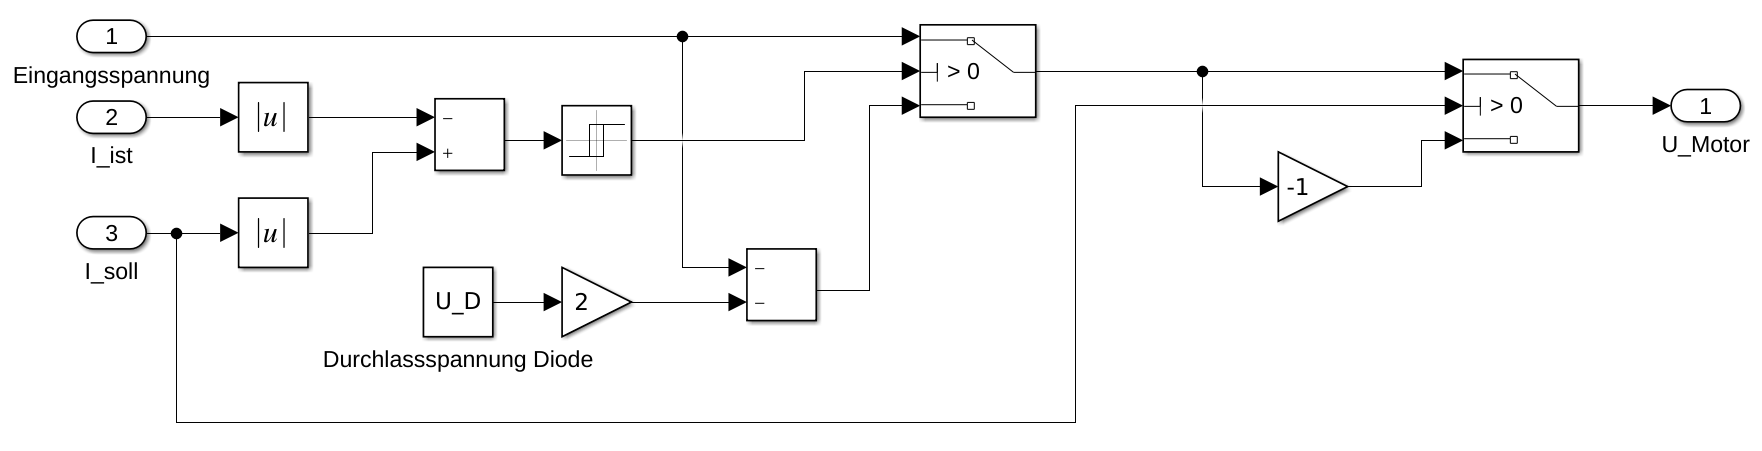
\includegraphics[width=1\textwidth]{hbridge_modell.png}
    \caption{Subsystem Steuerung mit H-Brücke}
    \label{fig:Subsystem H-Bridge}
\end{figure}

Das Subsystem beinhaltet Relay-Block der hier als Zweipunktregeler genutzt
wird. Die Beiden Schwellwerte $i_{plus}=10\mathrm{mA}$ und $i_{minus}=-10
\mathrm{mA}$ wurden im m-File definiert. Dieser gibt einen boolschen Wert
an den 1. Switch Block der zwischen Transistoren An und Aus hin- und
herschaltet. Der 2. Switch Block verändert die Drehrichtung des Motors und
wird geschaltet vom Vorzeichen des einzustellenden Strom $I_{soll}$.
\subsection{Zusammenfassung}

In diesem Versuch haben wir eine Steuerung mit H-Brücke modelliert und
sie mit dem Modell des Gleichstrommotor verbunden. Dieser lässt sich nun
Strom- statt Spannungs-gesteuert betreiben.
\section{Anhang}

\subsection{Aufgabenbeschreibung}
\begin{figure}[H]
    \centering
    \includegraphics[page=8, width=0.8\textwidth]{../Aufgabenstellung.pdf}
    %\caption{caption}
    \label{fig:Aufgabenstellung Labor 4.1}
\end{figure}

\begin{figure}[H]
    \centering
    \includegraphics[page=9, width=0.8\textwidth]{../Aufgabenstellung.pdf}
    \label{fig:Aufgabenstellung Labor 4.2}
\end{figure}

\subsection{Matlab Code}
\lstinputlisting[language=Matlab]{matlab/as_labor04_hbridge.m}

%\subsection{Messwerte}

\end{document}

\section{Einleitung und Ziel}

Im 4. Labor soll der zuvor modellierte, spannungsgesteuerte
Gleichstrommotor nun stromgesteuert werden. Dieses soll Mittels
eines Vierquadrantensteller auch H-Brücke genannt in Simulink
als Modell umgesetzt werden.



% \section{Einleitung und Ziel}

% Im 4. Labor im Modul Aktorik und Sensorik soll jubaefiubaefiu bestimmt werden.


% Was m"ussen Sie um das bestehende Motormodell hinzufügen, um einen Strom einprägen zu können?
% H-Br"ucke

% 2.1
% T_LH und T_RL

% 2.2 
% Durch die Drehung des Motors wird eine Spannung Induziert. Dadurch fließt ein Strom durch die 
% sogenannten Parasit"ardioden T_RH und T_LL. 

% 2.3
% Der Strom l"asst sich "uber R_shunt messen, welcher passenderweise mit 1 OHM gew"ahlt ist. So ist
% die Spannung, die an R_shunt abf"allt gleich des Stromes.

% 2.4
% Es gibt vier verschiedene Zust"ande. Wenn der Motor im Uhrzeigersinn betrieben werden soll, k"onnen
% die entsprechenden Transistoren geschaltet sein oder nicht geschaltet sein. Soll der Motor gegen
% den Uhrzeigersinn betrieben werden, kann das andere Transistorenpaar geschaltet sein oder nicht.

% 2.5
% Eing"ange: I_IST, I_Soll, U_H-Br"ucke
% Ausg"ange: U_Motor

% 2.6
% 1. Fall: AN
%     U_H = U_T_LH + U_Motor + U_T_RL + U_R_shunt

%     U_H = R_LH * I_m + (R_shunt * I_m)  

% 2. Fall: Aus
%     0 = U_H + U_D + U_Motor + U_D + U_shunt
\subsection{Grundlagen und Theorie}

Mit Hilfe einer sogenannten H-Brücke lassen sich die Wicklungen eines
Motors auf eine einfache Art und Weise ansteuern.\\

\begin{figure}[H]
    \centering
    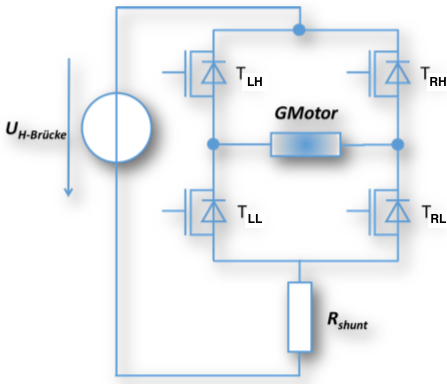
\includegraphics[width=1\textwidth]{schaltung_h_bruecke.png}
    \caption{Schaltung H-Brücke}
    \label{fig:Schaltung H-Bridge}
\end{figure}

Um den Strom positiv, also von links nach rechts, fließen zu lassen,
müssen die MOSFETS $T_{LH}$ und $T_{RL}$ angesteuert werden.\\

Wenn diese beiden besagten Transistoren ausgeschaltet werden, treibt die Energie im
Magnetfeld der Spule den Strom weiter. Dadurch fließt der Motorstrom $I_M$
durch die parasitären Bodydioden der Transistoren $T_{LL}$ und $T_{RH}$.\\

Dieser Strom kann indirekt durch die Spannung die über den Messwiderstand
$R_{Shunt}$ gemessen werden.\\

Soll der Motor in die entgegengesetzte Richtung betrieben werden, müssen
die MOSFETS $T_{RH}$ und $T_{LL}$ angesteuert werden.\\

Dadurch gibt es insgesamt 4 Zustände. Links-Rechts-Lauf Transistoren an oder
ausgeschaltet und Rechts-Links-Lauf Transistoren an oder ausgeschaltet.\\

Um die H-Brücke zu betreiben wird eine Steuerung benötigt. Die Steuerung
benötigt als Eingänge den Sollstrom $I_{soll}$, den momentanen Strom
$I_{ist}$ und die Eingangspannung. Als Ausgänge besitzt die Steuerung die
gepulste Motorspannung.\\

Die 4 Maschengleichung der 4 Zustände lauten wie folgt, wenn der
Drain-Source Widerstand vernachlässigt wird.\\

Link-Rechts-Lauf:

\begin{equation} \label{eq411}
    \begin{split}
        0 &= U_H - R \cdot i_M - L \cdot \dot{i_M} - k_e \cdot \omega - R_{Shunt} \cdot i_M\\
        0 &= U_H + 2 U_D + R \cdot i_M + L \cdot \dot{i_M} + k_e \cdot \omega + R_{Shunt} \cdot i_M
    \end{split}
\end{equation}

Rechts-Links-Lauf:

\begin{equation} \label{eq411}
    \begin{split}
        0 &= U_H + R \cdot i_M + L \cdot \dot{i_M} + k_e \cdot \omega - R_{Shunt} \cdot i_M\\
        0 &= U_H + 2 U_D - R \cdot i_M - L \cdot \dot{i_M} - k_e \cdot \omega + R_{Shunt} \cdot i_M
    \end{split}
\end{equation}


% 2.6
% 1. Fall: AN
%     U_H = U_T_LH + U_Motor + U_T_RL + U_R_shunt

%     U_H = R_LH * I_m + (R_shunt * I_m)  

% 2. Fall: Aus
%     0 = U_H + U_D + U_Motor + U_D + U_shunt
\subsection{Aufgabenstellung und Versuch}

Für das Subsystem Steuerung mit H-Brücke wurden folgenden Ein- und Ausgänge
definiert.\\

\begin{itemize}
    \item ($In_1$) Die Eingangs oder Betriebsspannung $U_H$
    \item ($In_2$) Der Momentanstrom $I_{ist}$
    \item ($In_3$) Der angestrebte Strom $I_{soll}$
    \item ($Out_1$) Die Spannung die über dem Motor abfällt $U_{Motor}$
\end{itemize}


\begin{figure}[H]
    \centering
    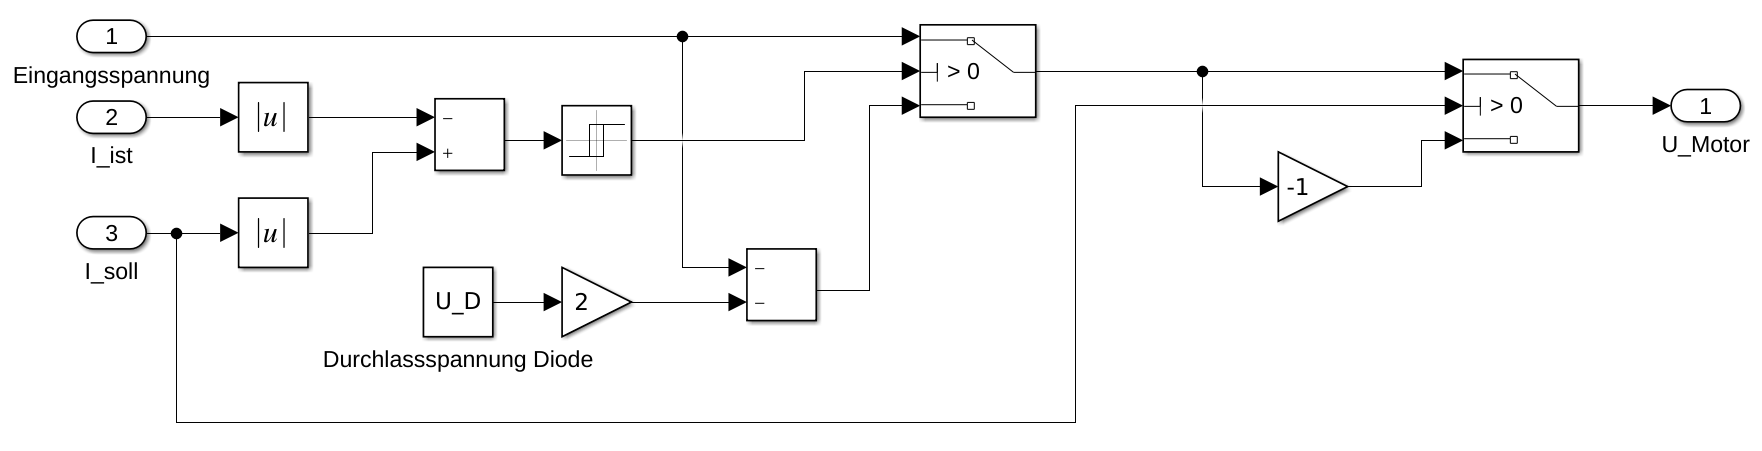
\includegraphics[width=1\textwidth]{hbridge_modell.png}
    \caption{Subsystem Steuerung mit H-Brücke}
    \label{fig:Subsystem H-Bridge}
\end{figure}

Das Subsystem beinhaltet Relay-Block der hier als Zweipunktregeler genutzt
wird. Die Beiden Schwellwerte $i_{plus}=10\mathrm{mA}$ und $i_{minus}=-10
\mathrm{mA}$ wurden im m-File definiert. Dieser gibt einen boolschen Wert
an den 1. Switch Block der zwischen Transistoren An und Aus hin- und
herschaltet. Der 2. Switch Block verändert die Drehrichtung des Motors und
wird geschaltet vom Vorzeichen des einzustellenden Strom $I_{soll}$.
\subsection{Zusammenfassung}

In diesem Versuch haben wir eine Steuerung mit H-Brücke modelliert und
sie mit dem Modell des Gleichstrommotor verbunden. Dieser lässt sich nun
Strom- statt Spannungs-gesteuert betreiben.
\section{Anhang}

\subsection{Aufgabenbeschreibung}
\begin{figure}[H]
    \centering
    \includegraphics[page=8, width=0.8\textwidth]{../Aufgabenstellung.pdf}
    %\caption{caption}
    \label{fig:Aufgabenstellung Labor 4.1}
\end{figure}

\begin{figure}[H]
    \centering
    \includegraphics[page=9, width=0.8\textwidth]{../Aufgabenstellung.pdf}
    \label{fig:Aufgabenstellung Labor 4.2}
\end{figure}

\subsection{Matlab Code}
\lstinputlisting[language=Matlab]{matlab/as_labor04_hbridge.m}

%\subsection{Messwerte}

\end{document}
